\documentclass[hyperref=unicode,presentation,10pt]{beamer}

\usepackage[absolute,overlay]{textpos}
\usepackage{array}
\usepackage{graphicx}
\usepackage{adjustbox}
\usepackage[version=4]{mhchem}
\usepackage{chemfig}
\usepackage{caption}

%dělení slov
\usepackage{ragged2e}
\let\raggedright=\RaggedRight
%konec dělení slov

\addtobeamertemplate{frametitle}{
	\let\insertframetitle\insertsectionhead}{}
\addtobeamertemplate{frametitle}{
	\let\insertframesubtitle\insertsubsectionhead}{}

\makeatletter
\CheckCommand*\beamer@checkframetitle{\@ifnextchar\bgroup\beamer@inlineframetitle{}}
\renewcommand*\beamer@checkframetitle{\global\let\beamer@frametitle\relax\@ifnextchar\bgroup\beamer@inlineframetitle{}}
\makeatother
\setbeamercolor{section in toc}{fg=red}
\setbeamertemplate{section in toc shaded}[default][100]

\usepackage{fontspec}
\usepackage{unicode-math}

\usepackage{polyglossia}
\setdefaultlanguage{czech}

\def\uv#1{„#1“}

\mode<presentation>{\usetheme{default}}
\usecolortheme{crane}

\setbeamertemplate{footline}[frame number]

\title[Crisis]
{C2062 -- Anorganická chemie II}

\subtitle{Skandium, yttrium, lanthanoidy a aktinoidy}
\author{Zdeněk Moravec, hugo@chemi.muni.cz \\ \adjincludegraphics[height=60mm]{img/IUPAC_PSP.jpg}}
\date{}

\begin{document}

\begin{frame}
	\titlepage
\end{frame}

\section{Úvod}
\frame{
	\frametitle{}
	\vfill
	\begin{tabular}{|l|l|l|l|l|}
	\hline
	 & \textit{Skandium} & \textit{Yttrium} & \textit{Lanthan} & \textit{Aktinium} \\\hline
	 El. k. & 3d$^{1}$ 4s$^{2}$ & 4d$^{1}$ 5s$^{2}$ & 5d$^{1}$ 6s$^{2}$ & 6d$^{1}$ 7s$^{2}$ \\\hline
	 T$_v$ [$^\circ$C] & 1541 & 1526 & 920 & 1227 \\\hline
	 T$_t$ [$^\circ$C] & 2836 & 2930 & 3464 & 3200 \\\hline
	 Objev & 1879 & 1794 & 1838 & 1899 \\\hline
	 & stříbrnobílý\footnote[frame]{Zdroj: \href{https://commons.wikimedia.org/wiki/File:Mscandium-3.jpg}{Commons}} & stříbrnobílý\footnote[frame]{Zdroj: \href{https://commons.wikimedia.org/wiki/File:Piece_of_Yttrium.jpg}{Jan Anskeit/Commons}} & stříbrnobílý\footnote[frame]{Zdroj: \href{https://commons.wikimedia.org/wiki/File:Lanthanum-2.jpg}{Jurii/Commons}} & stříbrnobílý\footnote[frame]{Zdroj: \href{https://commons.wikimedia.org/wiki/File:Actinium_sample_(31481701837).png}{Oak Ridge National Laboratory/Commons}} \\
	 & \begin{minipage}{.2\textwidth}
	 	\adjincludegraphics[width=\linewidth]{img/Mscandium-3.jpg}
	 \end{minipage}
	 	& \begin{minipage}{.2\textwidth}
	 		\adjincludegraphics[width=\linewidth]{img/Piece_of_Yttrium.jpg}
	 	\end{minipage} & \begin{minipage}{.2\textwidth}
	 	\adjincludegraphics[width=\linewidth]{img/Lanthanum-2.jpg} \end{minipage} & \begin{minipage}{.2\textwidth}
	 		\adjincludegraphics[width=\linewidth]{img/Actinium_sample.png}
 	\end{minipage} \\\hline
	\end{tabular}
	\vfill
}

\section{Chemické a fyzikální vlastnosti}
\frame{
	\frametitle{}
	\vfill
	\begin{itemize}
		\item Skandium yttrium, lanthan a lanthanoidy se označují jako \textit{kovy vzácných zemin}.
		\item Prvky mají lichá protonová čísla, proto vytvářejí více izotopů.
		\item Všechny mají stříbrnobílou barvu.
		\item Všechny na vzduchu za vyšší teploty hoří za vzniku oxidů \ce{M2O3}.
		\item Za laboratorní teploty reagují s halogeny, za vyšší teploty také s~většinou nekovů.
		\item S vodou reagují za vzniku vodíku, rychlost je možné zvýšit vyšší teplotou nebo zmenšením velikosti částic.
		\item Prvky vytvářejí převážně iontové sloučeniny v oxidačním čísle III.
		\item Nejméně bazickým iontem je nejmenší \ce{Sc^{3+}}. Chemicky je podobné hliníku.
		\item Lanthan a aktinium se svou zásaditostí blíží spíše vápníku.
		\item Všechny aktinoidy jsou radioaktivní prvky, nemají žádný stabilní izotop.
	\end{itemize}
	\vfill
	}

\section{Výskyt a získávání prvků}
\frame{
	\frametitle{}
	\vfill
	\begin{itemize}
		\item Kromě aktinia jde o poměrně rozšířené prvky.
		\item Aktinium je přítomno pouze ve stopovém množství v uranových rudách, kde vznikají radioaktivním rozpadem.
		\item Lanthanoidy jsou také poměrně rozšířené, je známo mnoho minerálů obsahujících tyto prvky.
		\item Jedinou výjimkou je \textit{promethium}, které nemá stabilní izotop ($^{147}$Pm, $t_{\frac{1}{2}}$ = 2,6 roku).
	\end{itemize}
	\begin{center}
		\begin{tabular}{|l|r@{,}l|l|r@{,}l|}
		\hline
		Prvek & \multicolumn{2}{l|}{[ppm]} & Prvek & \multicolumn{2}{l|}{[ppm]} \\\hline
		Ce & 66 & 0 & Tb & 1 & 2 \\\hline
		Pr & 9 & 1 & Dy & 4 & 5 \\\hline
		Nd & 40 & 0 & Ho & 1 & 4 \\\hline
		Pm & \multicolumn{2}{c|}{stopová množství} & Er & 3 & 5 \\\hline
		Sm & 7 & 0 & Tm & 0 & 5 \\\hline
		Eu & 2 & 1 & Yb & 3 & 1 \\\hline
		Gd & 6 & 1 & Lu & 0 & 8 \\\hline
	\end{tabular}
	\end{center}
	\vfill
}

\subsection{Skandium}
\frame{
	\frametitle{}
	\vfill
	\textbf{Skandium}
	\begin{columns}
	\begin{column}{0.7\textwidth}
		\begin{itemize}
			\item Roční produkce je okolo 20 tun, převážně oxidu skanditého. Poptávka je ale vyšší.
			\item Hlavním zdrojem jsou odpady vzniklé při zpracování uranových rud, příp. minerál \textit{thortveitit} (\ce{(Sc,Y)2Si2O7}).\footnote[frame]{\href{http://www.minsocam.org/ammin/AM73/AM73_601.pdf}{A re-examination of thortveitite}}
			\item Poprvé byl nalezen roku 1903, pojmenován byl roku 1911 po norském inženýrovi G.O. Olsenu Thortveitovi.\footnote[frame]{\href{http://webmineral.com/data/Thortveitite.shtml}{Thortveitite Mineral Data}}
			\item V roce 2004 byl nalezen průhledný exemplář v kvalitě odpovídající drahokamům.\footnote[frame]{\href{https://doi.org/10.15506/JoG.2008.31.1.1}{Thortveitite - a new gemstone}}
		\end{itemize}
	\end{column}
	\begin{column}{0.3\textwidth}
		\begin{figure}
			\adjincludegraphics[width=.92\textwidth]{img/Thortveitite.jpg}
			\caption*{Krystal thortveititu nalezený v Norsku.\footnote[frame]{Zdroj: \href{https://commons.wikimedia.org/wiki/File:Thortveitite-ea14a.jpg}{Robert M. Lavinsky/Commons}}}
		\end{figure}
	\end{column}
	\end{columns}
	\vfill
}

\subsection{Yttrium, lanthan}
\frame{
	\frametitle{}
	\vfill
	\textbf{Yttrium, lanthan}
	\begin{itemize}
		\item Oba prvky se získávají z nerostů.
		\item Dříve se produkty loužení minerálů v kyselině chlorovodíkové, sírové nebo hydroxidu sodném čistily frakční krystalizací. Tu ale bylo nutné mnohokrát opakovat.
		\item Dnes se využívají iontoměniče a speciální extrakční metody.
		\item Jednou z možností přípravy kovového yttria z oxidických rud je rozpuštění oxidu v kyselině sírové a následná frakcionace pomocí ionexové chromatografie.
		\item Přídavkem kyseliny šťavelové lze získat sraženinu šťavelanu yttritého, který se zahříváním rozkládá na oxid.
		\item Vzniklý oxid můžeme pomocí kyseliny fluorovodíkové převést na fluorid.
		\item \ce{Y2O3 + 6 HF -> 2 YF3 + 3 H2O}
	\end{itemize}
	\vfill
}

\frame{
	\frametitle{}
	\vfill
	\begin{itemize}
		\item \textit{Xenotim} je tetragonální minerál obsahující převážně fosforečnan yttritý, \ce{YPO4}.\footnote[frame]{\href{http://mineraly.sci.muni.cz/fosfaty/xenotim.html}{Xenotim}}
		\item Obsahuje přibližně 60~\% \ce{YPO4}.
		\item Největší důl je v Číně, v oblasti \textit{Bayan'obo Mining}.\footnote[frame]{\href{https://www.mindat.org/min-4333.html}{Xenotime-(Y)}}
	\end{itemize}
	\begin{columns}
		\begin{column}{.5\textwidth}
			\begin{figure}
				\adjincludegraphics[height=.35\textheight]{img/Xenotim_mineralogisches_museum_bonn.jpg}
				\caption*{Xenotim z Norska.\footnote[frame]{Zdroj: \href{https://commons.wikimedia.org/wiki/File:Xenotim_mineralogisches_museum_bonn.jpg}{Elke Wetzig Elya/Commons}}}
			\end{figure}
		\end{column}
		\begin{column}{.5\textwidth}
			\begin{figure}
				\adjincludegraphics[height=.35\textheight]{img/Xenotime_with_Rutile-08-2-78aa.jpg}
				\caption*{Xenotim s rutilem.\footnote[frame]{Zdroj: \href{https://commons.wikimedia.org/wiki/File:Xenotime_with_Rutile-08-2-78aa.jpg}{Robert M. Lavinsky/Commons}}}
			\end{figure}
		\end{column}
	\end{columns}
	\vfill
}

\frame{
	\frametitle{}
	\vfill
	\begin{itemize}
		\item Lanthan je třetím nejzastoupenějším lanthanoidem.
		\item Získává se z monazitových písků.
	\end{itemize}
	\begin{figure}
		\adjincludegraphics[width=.9\textwidth]{img/Monazite_acid_cracking_process.png}
		\caption*{Schéma zpracování monazitových písků.\footnote[frame]{Zdroj: \href{https://commons.wikimedia.org/wiki/File:Monazite_acid_cracking_process.svg}{Hydrargyrum/Commons}}}
	\end{figure}
	\begin{itemize}
		\item Kovový lanthan získáme z oxidu reakcí se salmiakem a následnou redukcí chloridu kovovým lithiem.
	\end{itemize}
	\begin{align*}
		\ce{La2O3 + 6 NH4Cl &-> 2 LaCl3 + 6 NH3 + 3 H2O} \\
		\ce{LaCl3 + 3 Li &->[vac] La + 3 LiCl}
	\end{align*}
	\vfill
}

\subsection{Lanthanoidy}
\frame{
	\frametitle{}
	\vfill
	\begin{itemize}
		\item S výjimkou promethia mají všechny lanthanoidy stabilní izotopy.
		\item V přírodě nejsou nijak vzácné.
		\item Nejvíce zastoupený je cer (46--60 mg/kg), nejméně pak lutecium (0,5--0,75 mg/kg).
		\item Známe více než 100 minerálů obsahujících lanthanoidy.
		\item \textit{Monazit} označuje skupinu fosfátových minerálů lanthanoidů.
		\item Přibližný vzorec: \ce{(Ce,La,Nd,Th)PO4}.\footnote[frame]{\href{http://mineraly.sci.muni.cz/fosfaty/monazit.html}{Monazit}}
		\item Složení se mění podle lokality, název určuje majoritní prvek, např. monazit-Ce.\footnote[frame]{\href{https://www.mindat.org/min-2751.html}{Monazite-(Ce)}}
		\item Jde o primární zdroj lanthanu a lanthanoidů.\footnote[frame]{\href{https://is.muni.cz/do/sci/UChem/um/spchp/ch20s01.html}{Lanthanoidy}}
	\end{itemize}
	\vfill
}

\frame{
	\frametitle{}
	\vfill
	\begin{columns}
		\begin{column}{.5\textwidth}
			\begin{figure}
				\adjincludegraphics[height=.55\textheight]{img/Monazite.jpg}
				\caption*{Monazit.\footnote[frame]{Zdroj: \href{https://commons.wikimedia.org/wiki/File:Monazite.JPG}{Sooo20036/Commons}}}
			\end{figure}
		\end{column}
		\begin{column}{.5\textwidth}
			\begin{figure}
				\adjincludegraphics[height=.55\textheight]{img/Monazite_sand.png}
				\caption*{Monazitový písek.\footnote[frame]{Zdroj: \href{https://commons.wikimedia.org/wiki/File:Monazite_sand.PNG}{D. Kemp, A. C. Cilliers/Commons}}}
			\end{figure}
		\end{column}
	\end{columns}
	\vfill
}

\frame{
	\frametitle{}
	\vfill
	\begin{itemize}
		\item \textit{Bastnezity} jsou skupinou minerálů obsahujících fluorid-uhličitan.\footnote[frame]{\href{https://www.mindat.org/min-563.html}{Bastnäsite-(Ce)}}
		\item Bastnezit-Ce: \ce{(Ce,La)CO3F}
		\item Bastnezit-La: \ce{(La,Ce)CO3F}
		\item Bastnezit-Y: \ce{(Y,Ce)CO3F}
	\end{itemize}
	\begin{columns}
		\begin{column}{.5\textwidth}
			\begin{figure}
				\adjincludegraphics[height=.32\textheight]{img/Bastnaesit_Burundi.jpg}
				\caption*{Bastnäsite z Burundi.\footnote[frame]{Zdroj: \href{https://commons.wikimedia.org/wiki/File:Bastnaesit_Burundi.jpg}{Kouame/Commons}}}
			\end{figure}
		\end{column}
		\begin{column}{.5\textwidth}
			\begin{figure}
				\adjincludegraphics[height=.32\textheight]{img/Bastnasite-122211.jpg}
				\caption*{Bastnäsite z Francie.\footnote[frame]{Zdroj: \href{https://commons.wikimedia.org/wiki/File:Bastnasite-122211.jpg}{Robert M. Lavinsky/Commons}}}
			\end{figure}
		\end{column}
	\end{columns}
	\vfill
}

\frame{
	\frametitle{}
	\vfill
	\begin{itemize}
		\item Zpracováním rud se získávají koncentráty s obsahem nad 90~\% minerálů vzácných zemin.
		\item Ty se rozloží buď pomocí kyselin nebo louhů a dále se zpracovávají.
		\item Konkrétní postup závisí na daném kovu, obecně je příprava čistých lanthanoidů velmi složitá a nákladná.
		\item Nejsnadněji lze izolovat cer, u něhož se využívá nižší bazicity ceričitých sloučenin oproti sloučeninám lanthanitým.
		\item Malá množství čistých prvků lze připravit pomocí iontoměničů, např. pomocí vytěsňovací chromatografie.
	\end{itemize}
	\begin{figure}
		\adjincludegraphics[width=0.35\textwidth]{img/Rareearthoxides.jpg}
		\caption*{Oxidy lantahnoidů.\footnote[frame]{Zdroj: \href{https://commons.wikimedia.org/wiki/File:Rareearthoxides.jpg}{Peggy Greb, US department of agriculture/Commons}}}
	\end{figure}
	\vfill
}

\frame{
	\frametitle{}
	\vfill
	\begin{itemize}
		\item $^{147}$Pm se získává štěpením $^{235}$U a $^{239}$Pu v reaktoru.\footnote[frame]{\scriptsize HÁLA, Jiří. \textit{Radioaktivní izotopy}. Tišnov: Sursum, 2013. ISBN 978-80-7323-248-1.}
		\item Rozpadá se za uvolnění částice $\beta^-$.
		\item \ce{^{147}Pm ->[t_{$\frac{1}{2}$} = 2,62 roku] ^{147}Sm + $\beta^-$}
		\item Promethium se sráží jako šťavelan promethitý, který je rozložen na oxid:
		\item \ce{Pm2(C2O4)3 ->[1000 $^\circ$C] Pm2O3 + 3 CO2 + 3 CO}
		\item Tento izotop se dříve využíval v radioizotopových bateriích kardiostimulátorů, elektřina byla generována absorpcí $\beta^-$ záření v křemíkovém PN přechodu.\footnote[frame]{\href{https://doi.org/10.1007/978-3-642-66187-7_25}{The Betavoltaic Pacemaker Power Source}}
		\item Baterie měly průměr 1,5--2,5~cm a výšku 1--2,5~cm, poskytovaly výkon 50--400~$\mu$W při napětí 1,5--4~V.
		\item Využívá se také pro kontinuální měření tloušťky plastů, pryže a papíru.
	\end{itemize}
	\vfill
}

\subsection{Aktinium}
\frame{
	\frametitle{}
	\vfill
	\begin{itemize}
		\item Aktinium se v přírodě vyskytuje pouze jako produkt rozpadu nestabilních jader.
		\item Uranové rudy obsahují přibližně 0,2~mg \ce{^{227}Ac} na tunu rudy:
		\item \ce{^{235}U ->[][-$\alpha$] ^{231}Th ->[][-$\beta$^-] ^{231}Pa ->[][-$\alpha$] ^{227}Ac}
		\item Thoriové rudy obsahují přibližně 5~ng \ce{^{228}Ac} na tunu rudy:
		\item \ce{^{232}Th ->[][-$\alpha$] ^{228}Ra ->[][-$\beta$^-] ^{228}Ac}
		\item Získávání aktinia z těchto rud je velmi obtížné, jak kvůli nízké koncentraci, tak i díky podobnosti s dalšími prvky. Proto se připravuje převážně uměle, ostřelováním jader radia neutrony:
		\item \ce{^{226}Ra + ^1_0n -> ^{227}Ra ->[$\beta$^-][2500 s] ^{227}Ac}
	\end{itemize}
	\vfill
}

\subsection{Aktinioidy}
\frame{
	\frametitle{}
	\vfill
	\begin{itemize}
		\item Všechny izotopy aktinoidů jsou nestabilní.
		\item Pouze čtyři izotopy mají dostatečně dlouhý poločas rozpadu, aby byly stále přítomny v přírodě.
		\item Tyto izotopy jsou součástí čtyř rozpadových řad:
		\begin{enumerate}
			\item Thoriová řada -- začíná $^{232}$Th a končí $^{208}$Pb
			\item Neptuniová řada -- začíná $^{237}$Np a končí $^{205}$Tl
			\item Uranová řada -- začíná $^{238}$U a končí $^{206}$Pb
			\item Aktiniová řada -- začíná $^{235}$U a končí $^{207}$Pb
		\end{enumerate}
	\end{itemize}
	\vfill
}

\frame{
	\frametitle{}
	\vfill
	\begin{columns}
		\begin{column}{.5\textwidth}
			\begin{figure}
				\adjincludegraphics[height=0.65\textheight]{img/Decay_Chain_Thorium.png}
				\caption*{Thoriová rozpadová řada.\footnote[frame]{Zdroj: \href{https://commons.wikimedia.org/wiki/File:Decay_Chain_of_Thorium.svg}{Tosaka/Commons}}}
			\end{figure}
		\end{column}

		\begin{column}{.5\textwidth}
			\begin{figure}
				\adjincludegraphics[height=0.65\textheight]{img/Decay_Chain_Neptunium.png}
				\caption*{Neptuniová rozpadová řada.\footnote[frame]{Zdroj: \href{https://commons.wikimedia.org/wiki/File:Decay_Chain(4n\%2B1,_Neptunium_Series).svg}{Tosaka/Commons}}}
			\end{figure}
		\end{column}
	\end{columns}
	\vfill
}

\frame{
	\frametitle{}
	\vfill
	\begin{columns}
		\begin{column}{.5\textwidth}
			\begin{figure}
				\adjincludegraphics[height=0.65\textheight]{img/Decay_Chain_Uranium.png}
				\caption*{Uranová rozpadová řada.\footnote[frame]{Zdroj: \href{https://commons.wikimedia.org/wiki/File:Decay_chain(4n\%2B2,_Uranium_series).svg}{Tosaka/Commons}}}
			\end{figure}
		\end{column}

		\begin{column}{.5\textwidth}
			\begin{figure}
				\adjincludegraphics[height=0.65\textheight]{img/Decay_Chain_Actinium.png}
				\caption*{Aktiniová rozpadová řada.\footnote[frame]{Zdroj: \href{https://commons.wikimedia.org/wiki/File:Decay_Chain_of_Actinium.svg}{Edgar Bonet/Commons}}}
			\end{figure}
		\end{column}
	\end{columns}
	\vfill
}

\frame{
	\frametitle{}
	\vfill
	\begin{itemize}
		\item Nejvyšší zastoupení v přírodě mají uran (16~ppm) a thorium (4~ppm).
		\item Z uranové rudy se loužením v kyselině sírové připraví solí \ce{UO$_2^{2+}$}, který je následně čištěn.
		\item Čistý \ce{UO2(NO3)2} se termicky rozloží na \ce{UO3}, který je redukován vodíkem.
		\item \ce{UO3 + H2 ->[700 $^\circ$C] UO2 + H2O}
		\item Oxid uraničitý je převeden na fluorid, který se redukuje hořčíkem.
		\item \ce{UO2 + 4 HF ->[500 $^\circ$C] UF4 + 2 H2O}
		\item \ce{UF4 + 2 Mg ->[700 $^\circ$C] U + 2 MgF2}
	\end{itemize}
	\vfill
}

\frame{
	\frametitle{}
	\vfill
	\begin{figure}
		\adjincludegraphics[height=0.7\textheight]{img/Uranium_production.png}
		\caption*{Světová produkce uranu v roce 2015.\footnote[frame]{Zdroj: \href{https://commons.wikimedia.org/wiki/File:Uranium_production,_OWID.svg}{Our World In Data/Commons}}}
	\end{figure}
	\vfill
}

\frame{
	\frametitle{}
	\vfill
	\begin{itemize}
		\item V Česku se uran těžil v Jáchymovských dolech v Krušných horách.
		\item Těžba uranu zde probíhala od roku 1853 až do roku 1964.\footnote[frame]{\href{http://www.prvky.com/tezba-uranu.html}{Historie těžby uranu v Krušných horách}}
		\item Další významnou oblastí byla Dolní Rožínka v okrese Žďár nad Sázavou.
		\item Zde probíhala hlubinná těžba od roku 1957 až do roku 2017.\footnote[frame]{\href{http://podzemi.solvayovylomy.cz/histhor/lokality/rozinka/rozinka.htm}{Uranové doly GEAM Dolní Rožínka}}
		\item V posledních letech se těžba pohybovala v rekordní hloubce až 1100~metrů.
	\end{itemize}
	\vfill
}

\frame{
	\frametitle{}
	\vfill
	\begin{figure}
		\adjincludegraphics[height=0.7\textheight]{img/Dolni-Rozinka.jpg}
		\caption*{Uranový důl v Dolní Rožínce.\footnote[frame]{Zdroj: \href{https://commons.wikimedia.org/wiki/File:Dolní-Rožínka-doly2013.jpg}{Ben Skála, Benfoto/Commons}}}
	\end{figure}
	\vfill
}

\frame{
	\frametitle{}
	\vfill
	\begin{columns}
		\begin{column}{.6\textwidth}
			\begin{itemize}
				\item Thorium se získává loužením monazitového písku v 73\% NaOH při teplotě 140~$^\circ$C.
				\item Suspenze hydratovaných oxidů je poté okyselena pomocí HCl až na pH 3,5.
				\item Sraženina \ce{ThO2} je pak rozpuštěna v kyselině dusičné a extrahována pomocí tributylfosfátu do petroleje.
				\item Kovové thorium se získává redukcí vápníkem nebo hořčíkem v argonové atmosféře.
			\end{itemize}
			\begin{figure}
				\adjincludegraphics[height=0.2\textheight]{img/OPOBu.png}
			\end{figure}
		\end{column}
		\begin{column}{.4\textwidth}
			\begin{figure}
				\adjincludegraphics[height=0.6\textheight]{img/Tor.jpg}
				\caption*{Thór, bůh hromu, deště, nebe a plodnosti země.\footnote[frame]{Zdroj: \href{https://commons.wikimedia.org/wiki/File:Thor\%27s_Fight_with_the_Giants_(Mårten_Winge)_-_Nationalmuseum_-_18253.tiff}{Nationalmuseum/Commons}}}
			\end{figure}
		\end{column}
	\end{columns}
	\vfill
}

\frame{
	\frametitle{}
	\vfill
	\begin{columns}
		\begin{column}{.65\textwidth}
			\begin{itemize}
				\item Plutonium bylo poprvé připraveno bombardováním $^{238}$U jádry deuteria v cyklotronu.\footnote[frame]{\href{https://discover.lanl.gov/publications/national-security-science/2021-winter/plutonium-timeline/}{Atomic number 94}}
				\item \ce{^{238}U + ^2H -> ^{238}Np + 2 n}
				\item \ce{^{238}Np -> ^{237}Np + $\beta$^-}
				\item Nejvýznamnějším izotopem je štěpitelný $^{239}$Pu, ten se připravuje dlouhodobým ozařováním uranu neutrony v reaktoru.
				\item \ce{^{238}U + n -> ^{239}U + $\gamma$}
				\item \ce{^{239}U -> ^{239}Pu + $\beta$^-}
				\item Izolace plutonia z vyhořelého paliva probíhá proces PUREX.
			\end{itemize}
		\end{column}

		\begin{column}{.45\textwidth}
			\begin{figure}
				\adjincludegraphics[width=\textwidth]{img/Plutonium3.jpg}
				\caption*{Plutonium.\footnote[frame]{Zdroj: \href{https://commons.wikimedia.org/wiki/File:Plutonium3.jpg}{U.S. Department of Energy/Commons}}}
			\end{figure}
		\end{column}
	\end{columns}
	\vfill
}

\section{Využití prvků}
\subsection{Skandium}
\frame{
	\frametitle{}
	\begin{itemize}
		\item Skandium nemá příliš velké využití.
		\item Asi hlavní aplikací je slitina skandia s hliníkem využívaná při konstrukci některých dílů letadel.\footnote[frame]{\href{https://doi.org/10.1007/s11837-003-0224-6}{The properties and application of scandium-reinforced aluminum}}
		\item Slitina \ce{Al20Li20Mg10Sc20Ti30} má hustotu 3,91~g.cm$^{-3}$ a velmi výhodné mechanické vlastnosti, srovnatelné s titanem.\footnote[frame]{\href{https://doi.org/10.1080/21663831.2014.985855}{A Novel Low-Density, High-Hardness, High-entropy Alloy with Close-packed Single-phase Nanocrystalline Structures}}
		\item Izotop $^{46}$Sc se rozpadá $\beta^-$ mechanismem s poločasem rozpadu 83,8~dní. To je velmi výhodné pro geologické účely, využívá se pro mapování pohybu písku, jílu a sedimentů na dně řek. Připravuje se ozařováním oxidu skanditého neutrony v reaktoru.\footnote[frame]{\scriptsize HÁLA, Jiří. \textit{Radioaktivní izotopy}. Tišnov: Sursum, 2013. ISBN 978-80-7323-248-1.}
		\item \ce{^{45}Sc + n -> ^{46}Sc + $\gamma$}
	\end{itemize}
}

\subsection{Yttrium}
\frame{
	\frametitle{}
	\begin{itemize}
		\item \textbf{Supravodiče}
		\item Kovy jsou dobrými vodiči elektrického proudu, jejich měrný odpor je při pokojové teplotě řádově $10^{-5}\ \Omega.cm$.
		\item Vodivost je převrácenou hodnotou odporu:
		\item $G = \frac{1}{R} = \frac{I}{U}\ \ [S = m^{-2} kg^{-1} s^3 A^2 = \Omega^{-1}]$
		\item Odpor vodiče lze vypočítat z hodnoty měrného odporu: $R = \rho \frac{l}{S}$
		\item Ohmův zákon: $R = \frac{U}{I}\ \ [\Omega = m^2.kg.s^{-3}.A^{-2}]$
		\begin{itemize}
			\item Vodič má odpor jeden ohm, jestliže po přiložení jednoho voltu napětí jím protéká proud jeden ampér.
		\end{itemize}
		\item Odpor vůči průtoku elektrického proudu je zpravidla nežádoucí vlastností materiálu.
		\item Elektrický odpor závisí na teplotě podle vztahu: $R = R_0(1 + \alpha\Delta t)$, kde $\alpha$ je teplotní součinitel elektrického odporu.
		\item V blízkosti absolutní nuly (0 K = $-$273,15 $^\circ$C) klesá odpor některých kovů a slitin na nulu, tyto se označují jako \textit{supravodiče}.
	\end{itemize}
}

\frame{
	\frametitle{}
	\begin{itemize}
		\item Supravodivost byla poprvé pozorována v roce 1911, Heike Kamerling-Onnes prováděl měření odporu rtuti za nízkých teplot.
		\item Při teplotě 4,2 K pozoroval vymizení elektrického odporu.
		\item K chlazení rtuti využíval kapalné helium.
	\end{itemize}
	\begin{figure}
		\adjincludegraphics[width=0.6\textwidth]{img/mercury-temp-res-1.png}
		\caption*{Závislost elektrického odporu rtuti na teplotě.}
	\end{figure}
}

\frame{
	\frametitle{}
	\begin{itemize}
		\item Jelikož nebylo možné měřit tak nízký odpor, využil pro jeho stanovení metodu měření magnetické indukce cívky ze supravodivého materiálu.
		\item \resizebox{0.3\textwidth}{!}{$B(t) = B(t_0)e^{-\frac{tR}{L}}$}
		\item Supravodivou cívku postupně vybudil proudem z vnějšího zdroje a potom ji uzavřel supravodivým drátem, tím vytvořil uzavřený obvod ze supravodivého materiálu a měřil pokles indukčnosti cívky.
		\item Stejná metoda se i dnes využívá pro buzení supravodivých cívek.
	\end{itemize}
	\begin{center}
		\adjincludegraphics[width=0.5\textwidth]{img/prvni-supravodic.png}
	\end{center}
}

\frame{
	\frametitle{}
	\begin{itemize}
		\item Supravodiče 1. typu -- kovy a polokovy, které jsou za laboratorní teploty vodivé.\footnote[frame]{\href{https://www.youtube.com/watch?v=h6FYs_AUCsQ}{The Physics of superconductors – video popisující základní princip supravodivosti}}
		\item Jejich supravodivost lze vysvětlit pomocí BCS teorie, ta tento jev vysvětluje vznikem \textit{Cooperových párů}. To jsou dvojice elektronů, které se chovají jako bosony a nikoliv jako leptony.
	\end{itemize}

	\begin{center}
		\begin{tabular}{|l|l||l|l|}
			\hline
			\textbf{Kov} & $T_C$ [K] & \textbf{Kov} & $T_C$ [K] \\\hline
			Pb & 7,196 & U & 0,20 \\\hline
			La & 4,88 & Hf & 0,128 \\\hline
			Ta & 4,47 & Ir & 0,1125 \\\hline
			Hg & 4,15 & Be & 0,023 \\\hline
			Sn & 3,72 & W & 0,0154 \\\hline
			In & 3,41 & Pt & 0,0019 \\\hline
			Tl & 2,38 & Rh & 0,000325 \\\hline
		\end{tabular}
	\end{center}
}

\frame{
	\frametitle{}
	\begin{itemize}
		\item Supravodiče 2. typu -- kovy, slitiny, oxidické materiály.
		\item Přechod do supravodivého stavu probíhá přes přechodový stav.
		\item Mají vyšší kritickou teplotu než supravodiče 1. typu.
	\end{itemize}

	\begin{center}
		\begin{tabular}{|l|l|}
			\hline
			\textbf{Kov} & $T_C$ [K] \\\hline
			\ce{YBa2Cu3O_{7-x}} & 95  \\\hline
			\ce{C60Cs2Rb} & 33  \\\hline
			\ce{Nb3Al} & 18  \\\hline
			\ce{Nb3Ge} & 23,3  \\\hline
			\ce{Nb3Sn} & 18,3  \\\hline
			NbTi & 10  \\\hline
		\end{tabular}
	\end{center}

	\begin{itemize}
		\item Supravodiče typu 1,5 -- vykazují znaky obou předchozích typů supravodičů.
		\item Tento typ supravodivosti byl poprvé pozorován u \ce{MgB2} v roce 2009.
		\item Chovají se, jako by byly složeny ze dvou supravodivých tekutin, které spolu interagují
	\end{itemize}
}

\frame{
	\frametitle{}
	\begin{columns}
		\begin{column}{.5\textwidth}
		\begin{itemize}
		\item \textbf{YBCO} -- \ce{YBa2Cu3O7}
		\item Skupina sloučenin vykazujících vysokoteplotní supravodivost, T$_c$ nad 77~K, tzn. nad teplotu varu kapalného dusíku.
		\item Mechanismus supravodivosti je složitější než u kovových supravodičů a dosud není zcela objasněn.
		\item Krystaluje v defektní perovskitové struktuře. Struktura se skládá z tetraedrů \ce{CuO4} propojených jednotkami \ce{CuO2}. Může tvořit i nestechiometrické fáze s nižším obsahem kyslíku.
		\end{itemize}
		\end{column}
		\begin{column}{.5\textwidth}
	\begin{figure}
		\adjincludegraphics[height=.65\textheight]{img/Ybco002.png}
		\caption*{Struktura YBCO.\footnote[frame]{Zdroj: \href{https://commons.wikimedia.org/wiki/File:Ybco002.svg}{Rswarbrick/Commons}}}
	\end{figure}
		\end{column}
	\end{columns}
}

\frame{
	\frametitle{}
	\begin{itemize}
		\item Lze je připravit poměrně jednoduchou syntézou:\footnote[frame]{\href{https://doi.org/10.1021/ed078p1182.1}{Superconductor Synthesis—An Improvement}}
		\item \small \ce{8 BaCO3 + 2 Y2(CO3)3 + 12 CuCO3 + 1-x O2 -> 4 YBa2Cu3O_{7-x} + 26 CO2}
		\item Výchozí látky se smísí v práškovém stavu a poté se kalcinují v atmosféře kyslíku.
	\end{itemize}
	\begin{figure}
		\adjincludegraphics[width=.8\textwidth]{img/BaYCusuperconduct.jpg}
		\caption*{Struktura YBCO.\footnote[frame]{Zdroj: \href{https://commons.wikimedia.org/wiki/File:BaYCusuperconduct.jpg}{Cadmium/Commons}}}
	\end{figure}
}

\frame{
	\frametitle{}
	\vfill
	\begin{itemize}
		\item \textbf{ReBCO} -- \ce{ReBa2Cu3O7} (Re = Rare-Earth, Sm, Nd a Gd)
		\item Yttrium je nahrazeno některým z prvků vzácných zemin.\footnote[frame]{\href{https://www.theengineer.co.uk/new-superconductors-raise-hope-for-fast-development-of-compact-fusion-reactor/}{New superconductors raise hope for fast development of compact fusion reactor}}
		\item Tyto supravodiče mají vysokou hodnotu kritické teploty i kritického pole, proto jsou to velmi perspektivní materiály pro vývoj reaktorů na jadernou fúzi.
		\item Lze z něj vyrábět jak dráty, tak i tenké filmy.
	\end{itemize}
	\begin{figure}
		\adjincludegraphics[height=.38\textheight]{img/NbTi3SnWire.jpg}
		\caption*{Ukázka supravodivých drátů.\footnote[frame]{Zdroj: \href{https://commons.wikimedia.org/wiki/File:NbTi3SnWire.jpg}{	Materialscientist/Commons}}}
	\end{figure}
	\vfill
}

\frame{
	\frametitle{}
	\begin{itemize}
		\item \textbf{Supravodivost za pokojové teploty}
		\item Zvyšování kritické teploty je velmi důležité pro aplikační možnosti supravodičů.
		\item Vyšších T$_c$ se zatím daří dosáhnout pouze za velmi vysokých tlaků.\footnote[frame]{\href{https://doi.org/10.12693/APhysPolA.138.715}{Phonon-Induced Superconducting State: From Metallic Hydrogen to \ce{LaH10}}}
		\item Jedním z možných materiálů je hydrid lanthanu \ce{LaH10} nebo LaXH (X = Sc, Y).\footnote[frame]{\href{https://doi.org/10.1038/s41598-020-58065-9}{From \ce{LaH10} to room–temperature superconductors}}
	\end{itemize}
	\vfill
}

\frame{
	\frametitle{}
	\begin{itemize}
		\item V roce 1933 studovali němečtí fyzici Walther Meissner a Robert Ochsenfeld rozložení magnetického pole v okolí cínu a olova v supravodivém stavu.
		\item Zjistili, že supravodiče se chovají jako ideální diamagnetika, tzn. že ze svého objemu vypuzují magnetické pole.
		\item To umožňuje supravodičům odpuzovat magnety a chovat se jako magnetický štít s velmi velkou účinností.
		\item Tento jev označujeme jako \textit{Meisnerův-Oschsenfeldův efekt}.
		\item Můžeme ho popsat Londonovými rovnicemi:
		\item $\frac{\partial \mathbf{j}_{s}}{\partial t} = \frac{n_{\rm s} e^2}{m}\mathbf{E}, \nabla \times\mathbf{j}_{s} =-\frac{n_{\rm s} e^2}{m }\mathbf{B}$
	\end{itemize}
}

\frame{
	\frametitle{}
	\begin{columns}
		\begin{column}{.5\textwidth}
			\begin{figure}
				\adjincludegraphics[height=.75\textwidth]{img/EfektMeisnera.png}
				\caption*{Interakce magnetického pole se supravodičem.\footnote[frame]{Zdroj: \href{https://commons.wikimedia.org/wiki/File:EfektMeisnera.svg}{Piotr Jaworski/Commons}}}
			\end{figure}
		\end{column}

		\begin{column}{.5\textwidth}
			\begin{figure}
				\adjincludegraphics[height=.75\textwidth]{img/Meissner_effect.jpg}
				\caption*{Meissnerův efekt.\footnote[frame]{Zdroj: \href{https://commons.wikimedia.org/wiki/File:Meissner_effect_p1390048.jpg}{Mai-Linh Doan/Commons}}}
			\end{figure}
		\end{column}
	\end{columns}
}

\frame{
	\frametitle{}
	\begin{itemize}
		\item \textit{NMR - Nukleární Magnetická Rezonance.}
		\item Technika využívaná ke zobrazení vnitřních orgánů
		\item Sledujeme absorpci radiofrekvenčního záření vzorkem, který je umístěn v magnetickém poli.
		\item Vzorek je nejčastěji kapalný, ale lze měřit i pevné látky a plyny.
		\item Jde o důležitou metodu v chemické a strukturní analýze.
		\item Vyžaduje silné magnetické pole, proto se nejčastěji využívá supravodivých magnetů.
	\end{itemize}
}

\frame{
	\frametitle{}
	\vfill
	\begin{itemize}
		\item Atomové jádro se skládá z protonů a neutronů.
		\item Obě částice mají spin $\pm\frac{1}{2}$.
		\item Jaderný spin je roven součtu spinů všech nukleonů.
		\item V NMR jsou aktivní pouze jádra s \emph{nenulovým jaderným spinem}.
		\item Nejčastěji se využívají jádra se spinem $\frac{1}{2}$, např. $^1$H, $^{13}$C, $^{19}$F nebo $^{31}$P.
		\item Bez vlivu vnějšího magnetického pole mají všechny orientace jaderného spinu stejnou energii.
		\item Pokud ale vložíme jádro do magnetického pole, získáme systém hladin o různých energiích.
		\item Pokud na tento systém působíme radiofrekvenčním zářením, může dojít k absorpci energie a excitaci spinu na vyšší energetickou hladinu.
		\item Poté pozorujeme návrat spinu a původní hladinu a emisi absorbované energie, kterou následně snímáme.
	\end{itemize}
	\vfill
}

\frame{
	\frametitle{}
	\vfill
	\begin{center}
		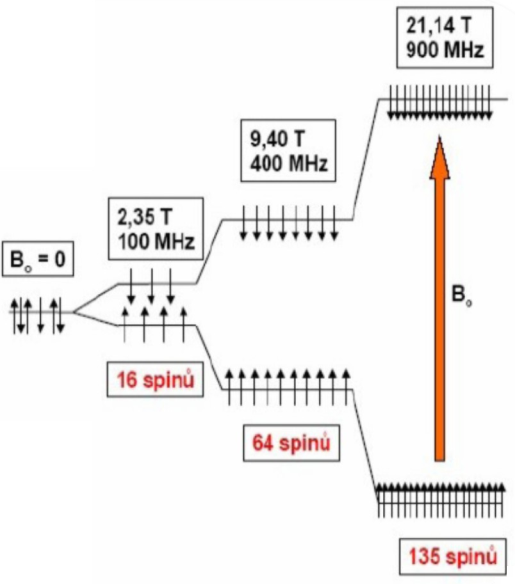
\includegraphics[keepaspectratio,width=7cm]{img/NMR-levels.png}
	\end{center}
	\vfill
}

\frame{
	\frametitle{}
	\vfill
	\begin{itemize}
		\item FT-NMR využívá k excitaci jaderných spinů radiofrekvenční pulsy.
		\item Ty excitují všechna měřená jádra, např. protony, najednou.
		\item Pulsy sklápí vektor magnetizace a způsobují jeho precesi.
		\item Délka pulsů se pohybuje v řádu $\mu$s.
		\item Čím je puls delší, tím je větší i sklápěcí úhel.\footnote[frame]{\href{https://nmr.chem.ucsb.edu/protocols/pw90cal.html}{~$^1$H 90 degree pulse width calibration}}
	\end{itemize}
	\begin{center}
		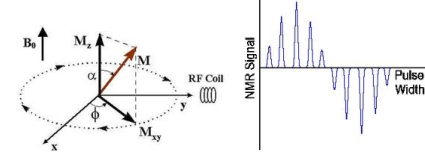
\includegraphics[keepaspectratio,width=.65\textwidth]{img/NMR-pulse.png}
	\end{center}
	\vfill
}

\frame{
	\frametitle{}
	\vfill
	\begin{itemize}
		\item Izolovaná jádra stejného izotopu budou v magnetickém poli rezonovat při stejné frekvenci.
		\item Pokud uvažujeme molekuly, je každé jádro ovlivněno také lokálními magnetickými poli, které jsou generovány vazebnými elektrony. Tím dochází ke změně rezonanční frekvence daného jádra.
		\item Změna je dána tzv. chemickým okolím pozorovaného jádra a nazývá se \emph{chemický posun}. Označuje se $\delta$ a je dán vztahem:
	\end{itemize}
	\begin{center}
		$\delta = \frac{\nu - \nu_{TMS}}{\nu}$
	\end{center}
	\begin{itemize}
		\item $\nu_{TMS}$ je rezonanční frekvence standardu, $\nu$ je rezonanční frekvence signálu.
		\item Chemický posun je bezrozměrný, jelikož se jedná o velmi malé hodnoty, udává se v ppm.
		\item Chemický posun je, na rozdíl od rezonanční frekvence, nezávislý na hodnotě vnějšího magnetického pole.
	\end{itemize}
	\vfill
}

\frame{
	\frametitle{}
	\vfill
	\begin{columns}
		\begin{column}{.6\textwidth}
			\textbf{Lanthanoidová posuvová činidla}
	\begin{itemize}
		\item Problémem $^1$H NMR je malý interval chemických posunů ($-$2--20~ppm), proto často dochází k překryvu signálů.
		\item Jednou možností, jak překryv řešit je použití silnějšího NMR magnetu, to je ale ekonomicky nákladné.
		\item Další možností je využít komplexy lanthanoidů ke změně hodnoty chemického posunu některých signálů.\footnote[frame]{\href{https://doi.org/10.1021/cr60286a001}{Lanthanide shift reagents for nuclear magnetic resonance spectroscopy}}
		\item Ionty lanthanoidů se chovají jako Lewisovy kyseliny a interagují s bazickými centry v molekule vzorku. Tím dochází ke změně chemického posunu daného signálu.
	\end{itemize}
		\end{column}
	\begin{column}{.4\textwidth}
		\begin{figure}
			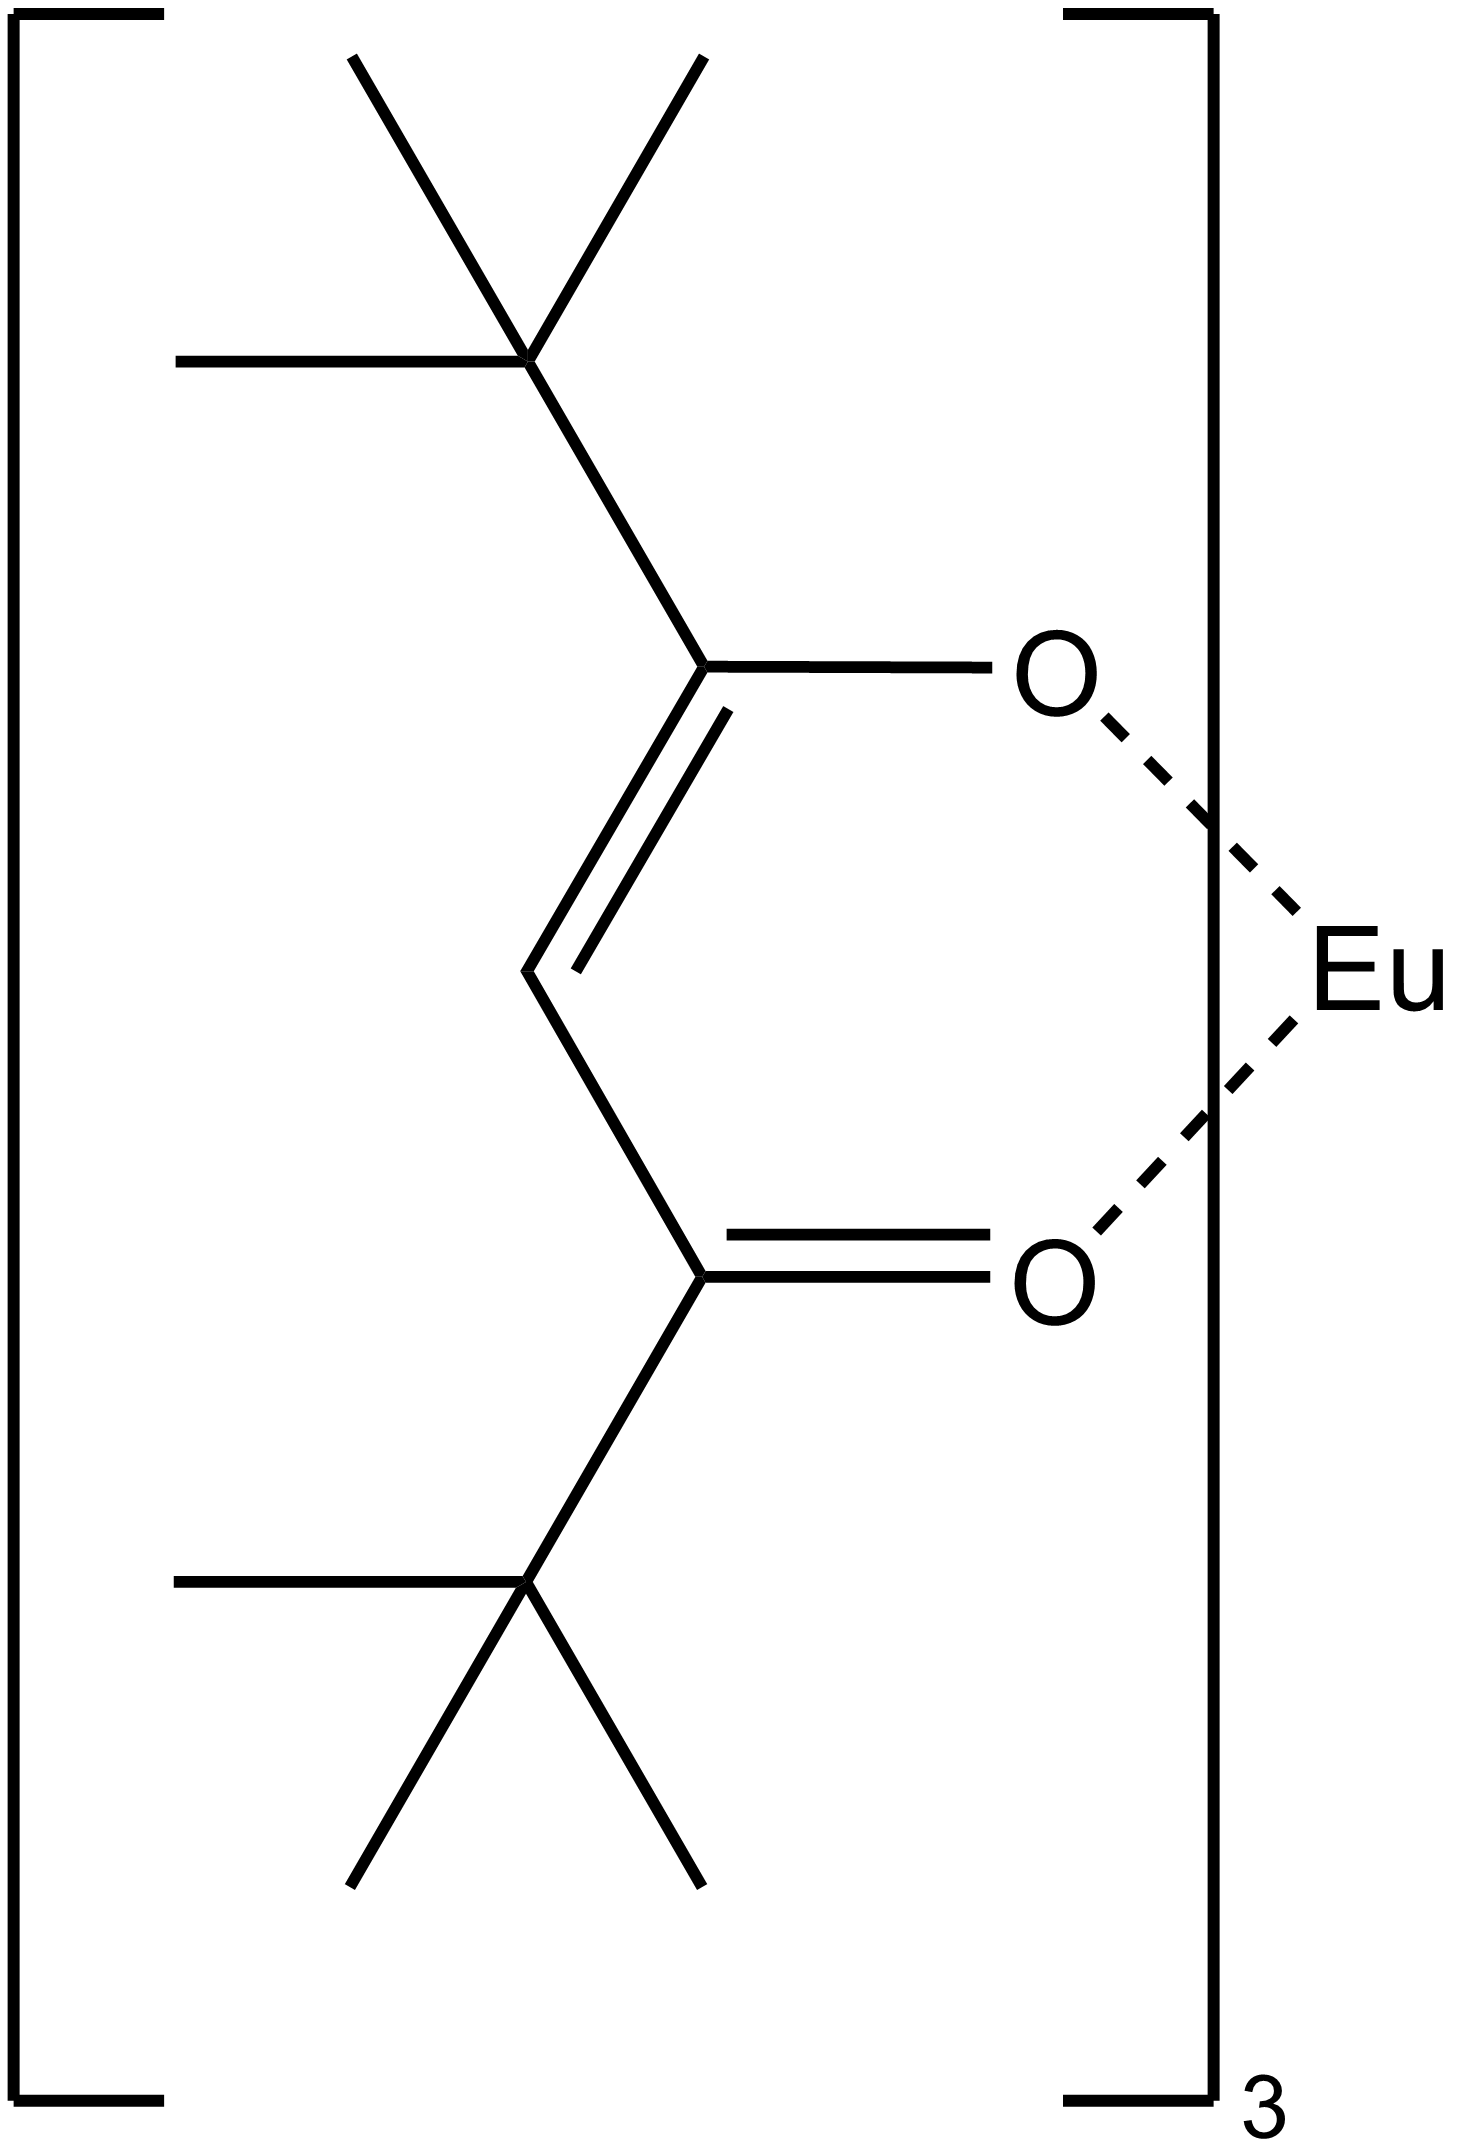
\includegraphics[keepaspectratio,width=\textwidth]{img/Eu-dpm.png}
		\end{figure}
	\end{column}
	\end{columns}
	\vfill
}

\frame{
	\frametitle{}
	\vfill
	\begin{itemize}
		\item Pokud je v molekule více NMR aktivních jader, může docházet k jejich vzájemné interakci. Síla této interakce je dána hlavně počtem vazeb, které jádra oddělují.
		\item Velikost interakční konstanty je nezávislá na intenzitě magnetického pole.
	\end{itemize}
	\begin{center}
		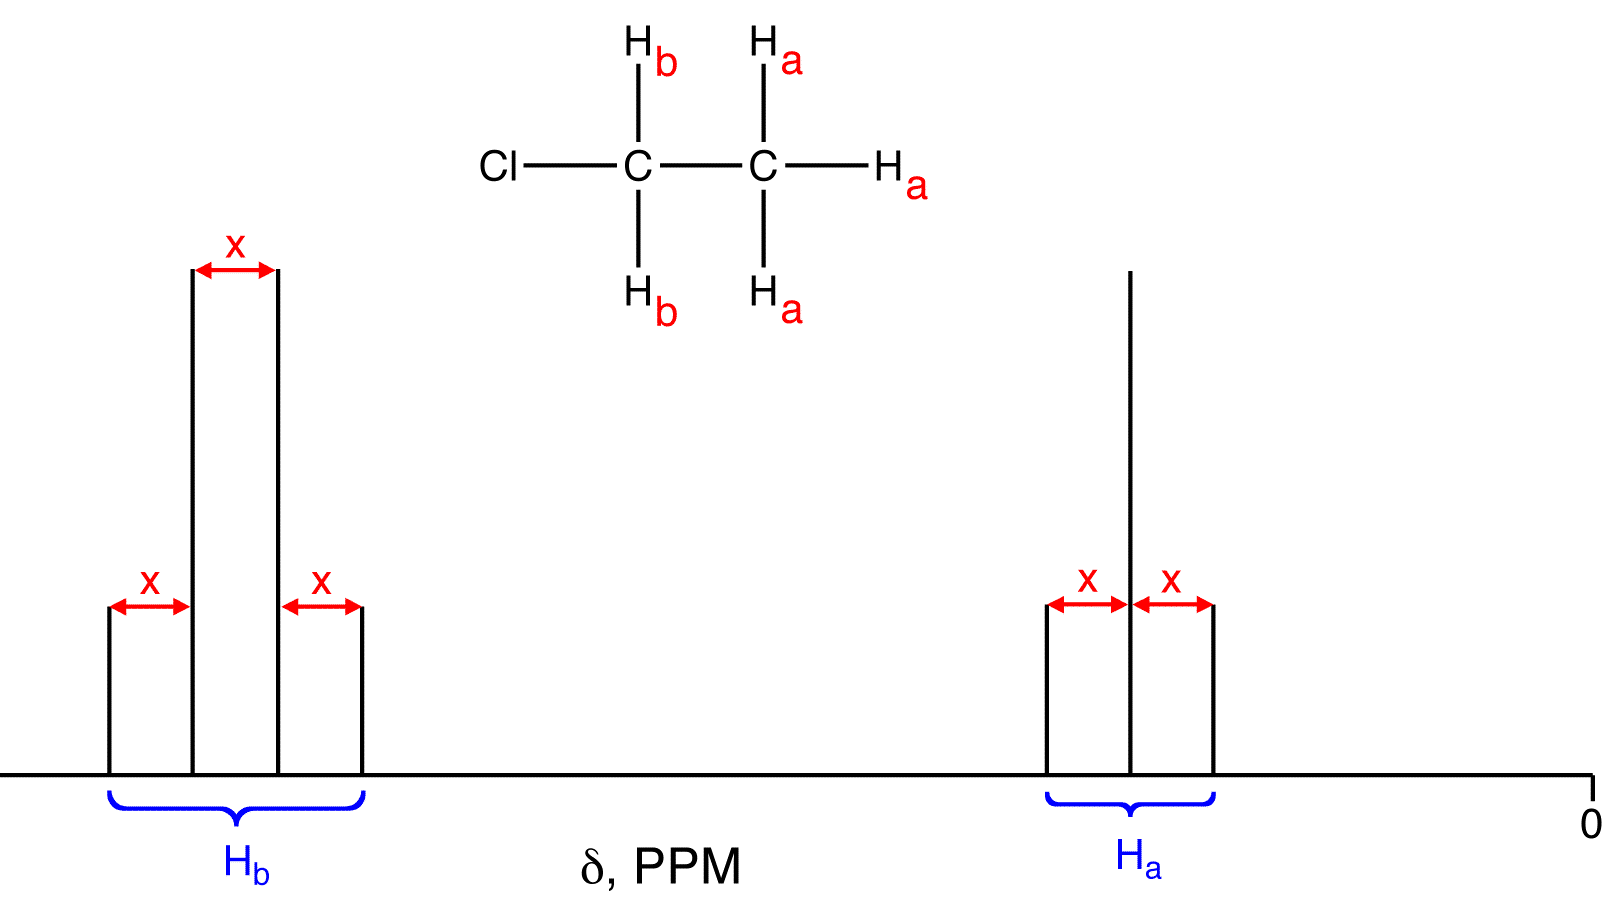
\includegraphics[keepaspectratio,width=9cm]{img/couplingconstant.png}
	\end{center}
	\vfill
}

\frame{
	\frametitle{}
	\vfill
	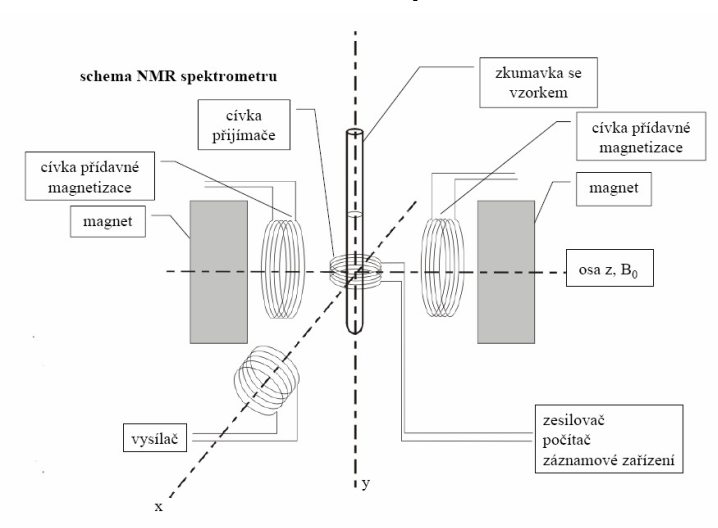
\includegraphics[keepaspectratio,width=10cm]{img/NMR-blockScheme.png}
	\vfill
}

\frame{
	\frametitle{}
	\vfill
	\begin{itemize}
		\item Permanentní magnety (Halbachovy) - do 100 MHz
	\end{itemize}
	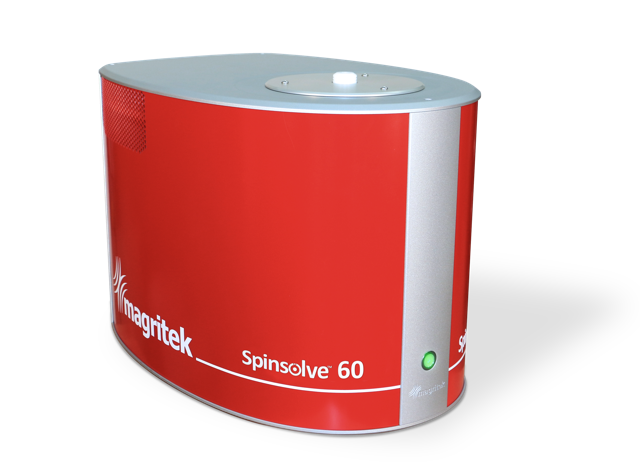
\includegraphics[keepaspectratio,width=10cm]{img/NMR-Magritek.png}
	\vfill
}

\frame{
	\frametitle{}
	\vfill
	\begin{itemize}
		\item Cryogen-free magnety - 100-300 MHz - levný provoz
	\end{itemize}
	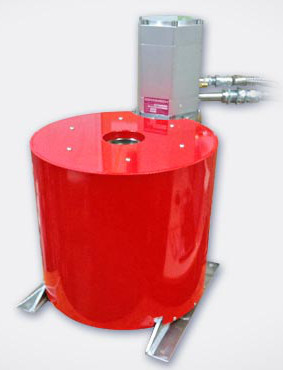
\includegraphics[keepaspectratio,width=5cm]{img/200mhz cryogenfree.jpg}
	\vfill
}

\frame{
	\frametitle{}
	\vfill
	\begin{itemize}
		\item Supravodivé magnety - nejběžnější v NMR
		\begin{itemize}
			\item Chlazené kapalným heliem (4-2,2 K)
			\item Magnetické pole až 28,2 T (1200 MHz)\footnote[frame]{\href{https://cen.acs.org/business/instrumentation/Bruker-installs-12-GHz-NMR/98/i19}{Bruker installs world's first 1.2 GHz}}
		\end{itemize}
	\end{itemize}
	\begin{figure}
		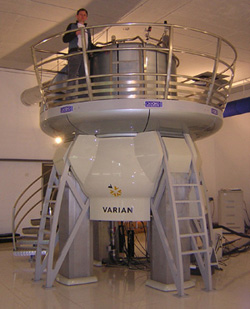
\includegraphics[height=.5\textheight]{img/Varian-_900MHz_-_21.2_Tesla.jpg}
		\caption*{NMR magnet 900 MHz.\footnote[frame]{Zdroj: \href{https://commons.wikimedia.org/wiki/File:HWB-NMR_-_900MHz_-_21.2_Tesla.jpg}{MartinSaunders/Commons}}}
	\end{figure}
	\vfill
}

\frame{
	\frametitle{}
	\vfill
	\begin{figure}
		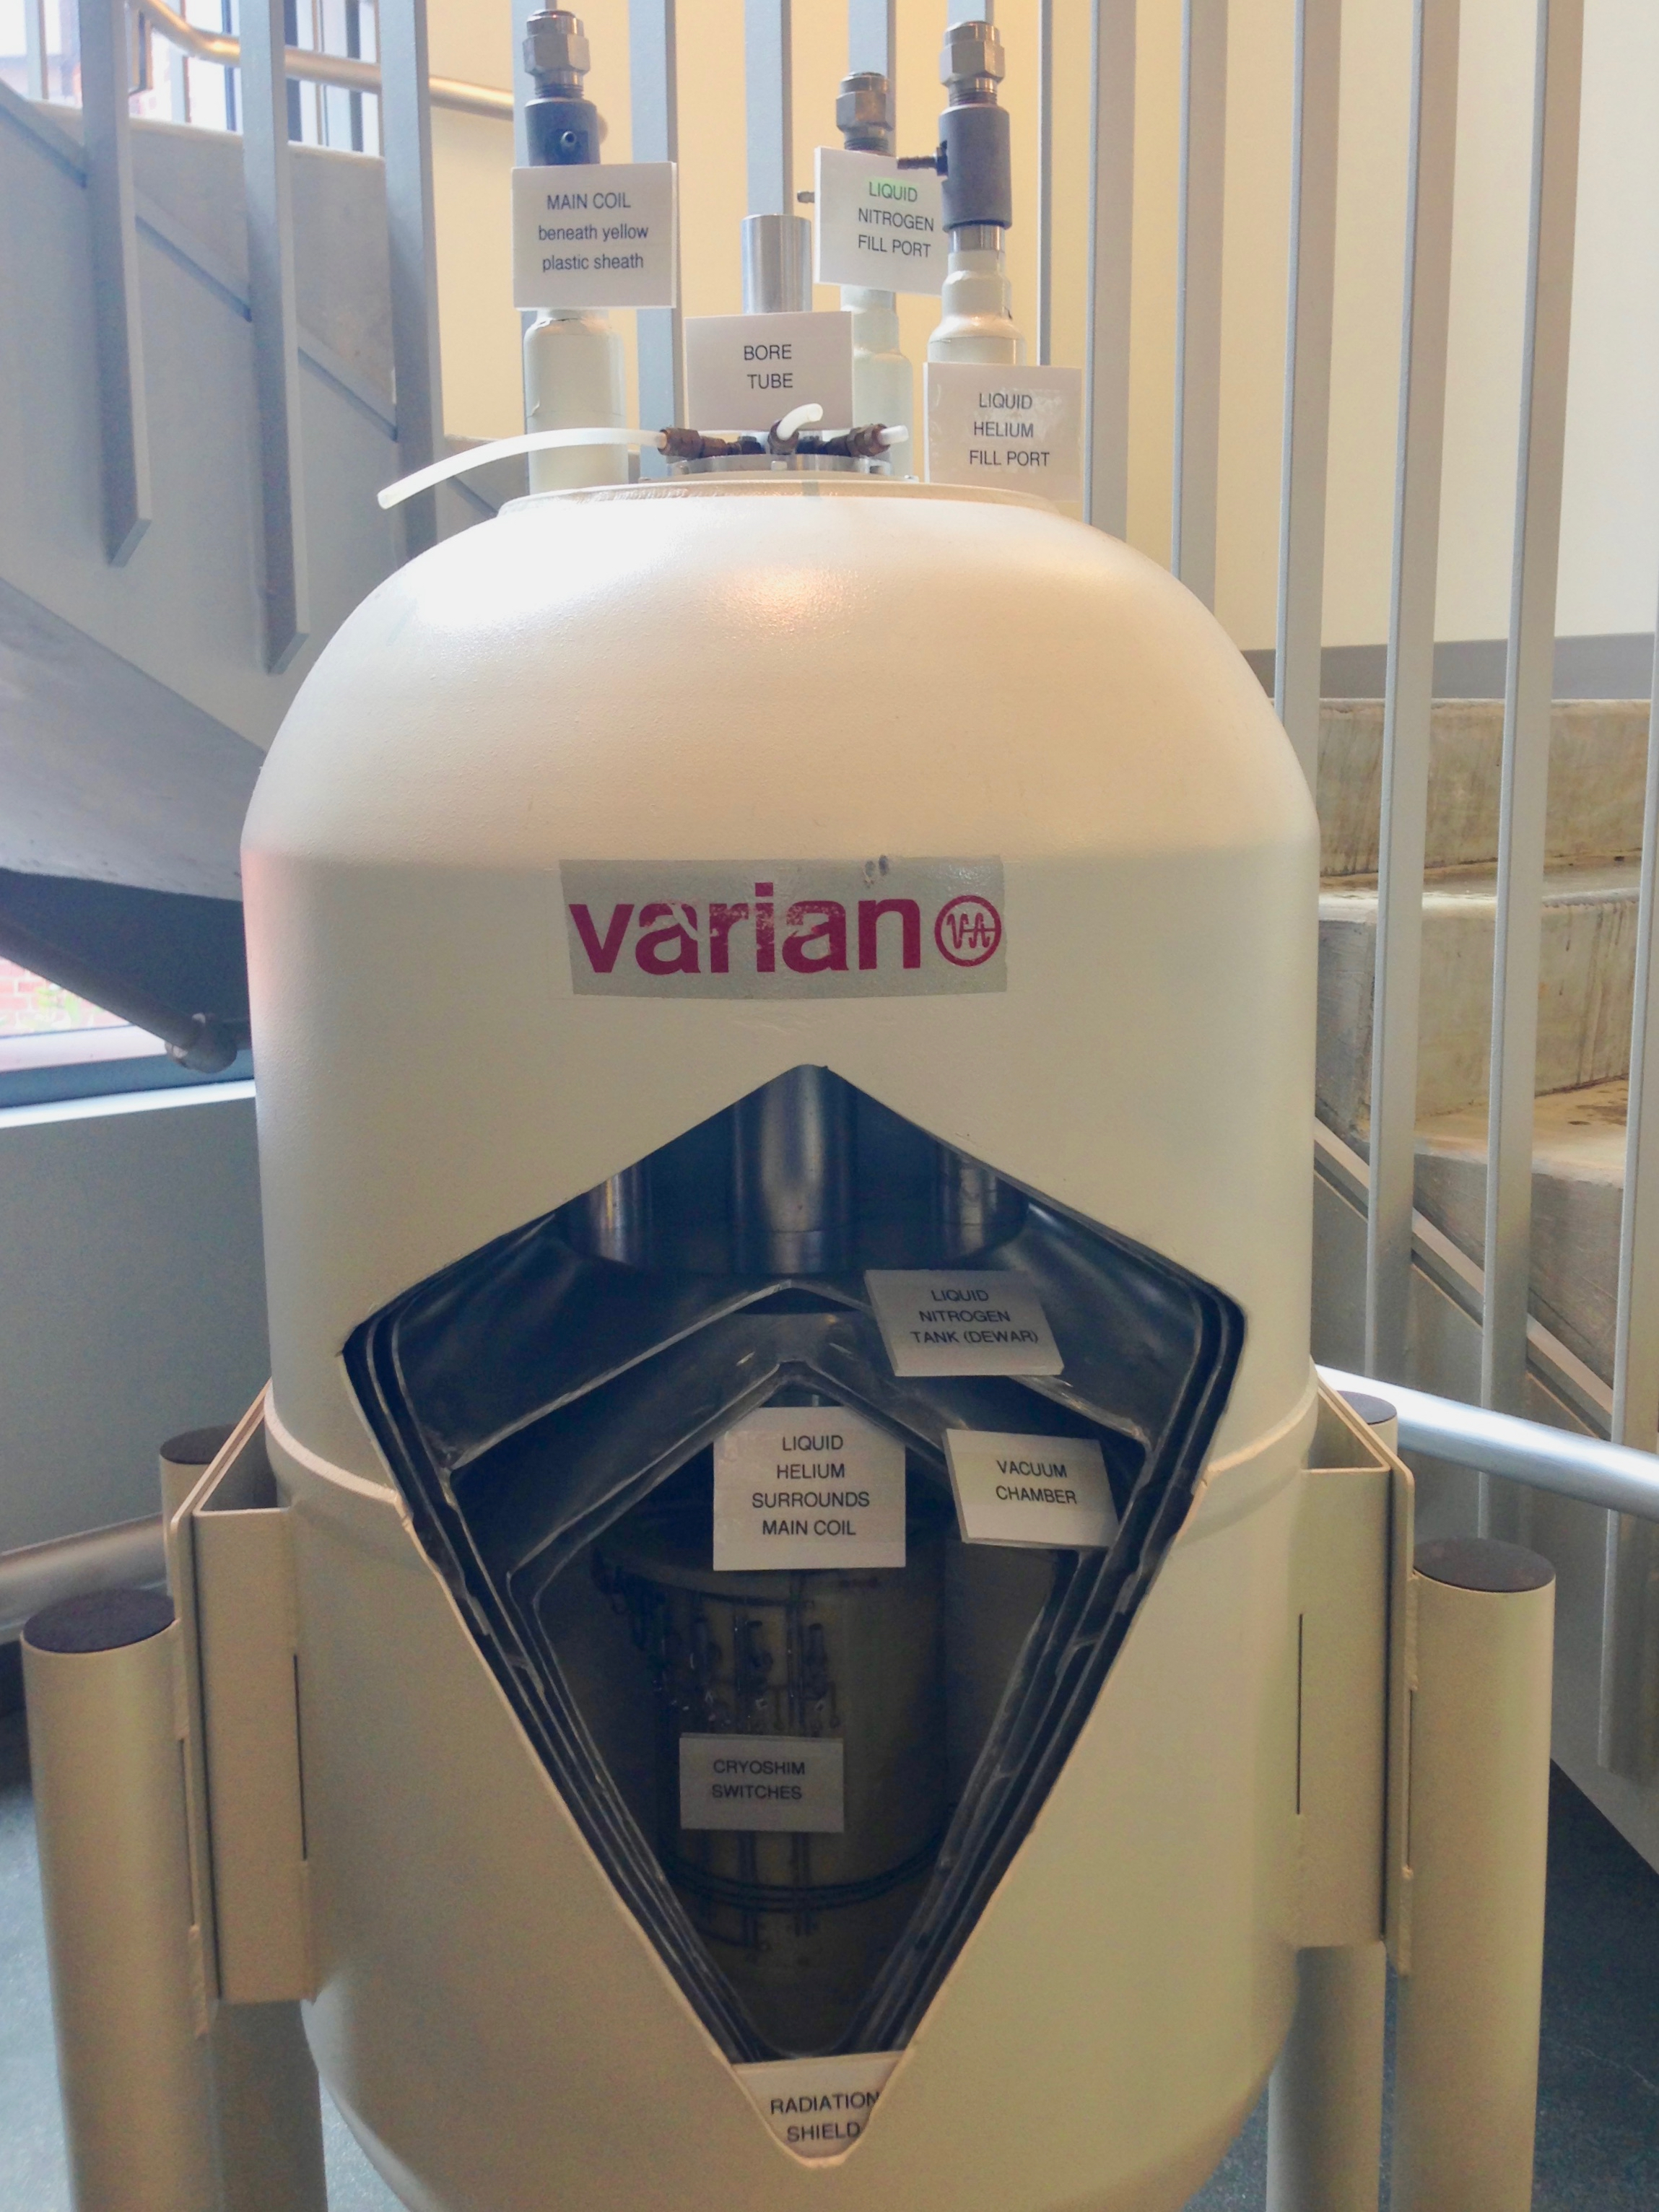
\includegraphics[keepaspectratio,height=0.7\textheight]{img/Cutaway_of_NMR_magnet.jpg}
		\caption*{Řez NMR magnetem.\footnote[frame]{Zdroj: \href{https://commons.wikimedia.org/wiki/File:Cutaway_of_NMR_magnet.jpg}{Z22/Commons}}}
	\end{figure}
	\vfill
}

\frame{
	\frametitle{}
	\begin{tabular}{|l|l|l|}
		\hline
		$B_0$ [T] & $^1H$ [MHz] & $^{13}C$ [MHz] \\\hline
		1,41 & 60 & 15,1 \\\hline
		2,35 & 100 & 25,15 \\\hline
		7,05 & 300 & 75,4 \\\hline
		11,74 & 500 & 125,7 \\\hline
		14,09 & 600 & 150,9 \\\hline
		16,44 & 700 & 176,05 \\\hline
		19,97 & 850 & 213,78 \\\hline
		22,32 & 950 & 238,94 \\\hline
		28,2 & 1200 & 301,89 \\\hline
	\end{tabular}
	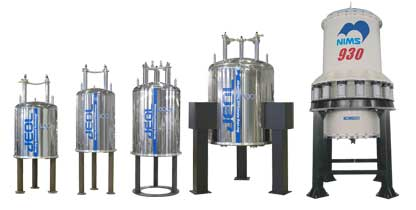
\includegraphics[keepaspectratio,width=5cm]{img/JEOL_NMR-Magnets_Family.jpg}
}

\frame{
	\frametitle{}
	\vfill
	\begin{itemize}
		\item \textit{MRI} - Magnetic Resonance Imaging
		\item Technika využívaná ke zobrazení vnitřních orgánů.
		\item Na rozdíl od NMR neměříme chemický posun, ale rozdílné relaxační časy vodíkových jader v organismu.
	\end{itemize}

	\begin{columns}
		\begin{column}{.5\textwidth}
			\begin{figure}
				\adjincludegraphics[height=4cm]{img/MRI-Philips.JPG}
				\caption*{MRI přístroj.\footnote[frame]{Zdroj: \href{https://commons.wikimedia.org/wiki/File:MRI-Philips.JPG}{Jan Ainali/Commons}}}
			\end{figure}
		\end{column}
		\begin{column}{.5\textwidth}
			\begin{figure}
				\adjincludegraphics[height=4cm]{img/MRI_knee_abdonrmal.jpg}
				\caption*{Snímek z MRI.\footnote[frame]{Zdroj: \href{https://commons.wikimedia.org/wiki/File:MRI_knee_abdonrmal.jpg}{Ptrump16/Commons}}}
			\end{figure}
		\end{column}
	\end{columns}

	\vfill
}

\frame{
	\frametitle{}
	\vfill
	\begin{itemize}
		\item \textit{MAGLEV} –- vlak pohybující se na vzduchovém polštáři.
		\item Využívá principu MAGnetické LEVitace, které je dosahováno pomocí supravodivých cívek.
		\item Příkladem může být pozemní dráha v Šanghaji o délce asi 40~km. Vlaky na ní dosahují rychlosti až 431~km/h.
	\end{itemize}
	\begin{columns}
		\begin{column}{.5\textwidth}
			\begin{figure}
				\adjincludegraphics[height=35mm]{img/Meissner_effect.jpg}
				\caption*{Levitace magnetu nad supravodičem.\footnote[frame]{Zdroj: \href{https://commons.wikimedia.org/wiki/File:Meissner_effect_p1390048.jpg}{Mai-Linh Doan/Commons}}}
			\end{figure}
		\end{column}
		\begin{column}{.5\textwidth}
			\begin{figure}
				\adjincludegraphics[height=35mm]{img/Maglev_june2005.jpg}
				\caption*{Maglev.\footnote[frame]{Zdroj: \href{https://commons.wikimedia.org/wiki/File:Maglev_june2005.jpg}{JakeLM/Commons}}}
			\end{figure}
		\end{column}
	\end{columns}
	\begin{center}


	\end{center}
	\vfill
}

\frame{
	\frametitle{}
	\vfill
	\textbf{Energetika}
	\begin{tabular}{|l|l|l|}
		\hline
		\textbf{Země} & \textbf{Spotřeba [TWh]} & \textbf{Spotřeba na hlavu [MWh]} \\\hline
		Čína & 4 830 & 3,56 \\\hline
		USA & 4 070 & 12,96 \\\hline
		Indie & 940 & 0,76 \\\hline
		Německo & 585 & 7,14 \\\hline
		Svět & 20 900 & 2,97 \\\hline
	\end{tabular}
	\begin{itemize}
		\item Očekávaná spotřeba v roce 2040 činí 40 000 TWh.
		\item K výrazným ztrátám dochází při transportu energie, důvodem je odpor kovů tvořících vedení.
		\item Ztrátový výkon můžeme vypočítat pomocí vztahu pro výkon a Ohmova zákona:
		\item $P_Z = UI = R . I . I = RI^2$
		\item Minimalizovat ztráty lze zmenšením odporu vedení nebo proudu.
		\item V současnosti se pro přenos na velké vzdálenosti využívá vedení VVN, tj. 110 kV.
		\item Zcela eliminovat ztráty by bylo možné s využitím supravodivých vodičů.
	\end{itemize}
	\vfill
}

\frame{
	\frametitle{}
	\vfill
	\begin{columns}
		\begin{column}{.75\textwidth}
			\begin{itemize}
				\item \textit{Jaderná fůze}
				\item Místo štěpení těžkých jader, dochází ke slučování lehkých jader.
				\item Nejvýhodnější je využití izotopů vodíku, které se slučují za vzniku jader helia a uvolnění energie.
				\begin{itemize}
					\item \ce{^2_1H + ^3_1H -> ^4_2He + ^1_0n}
				\end{itemize}
				\item Aby ke slučování mohlo dojít, je nutné v místě reakce vytvořit plasma o teplotě 100 miliónů $^\circ$C.\footnote[frame]{\href{https://www.aldebaran.cz/zvuky/blyskani/docs/10.html}{Zapálíme Slunce na Zemi?}}
				\item Gram směsi deuteria s tritiem by měl být schopen generovat výkon 500 MW po dobu asi jedné minuty.
			\end{itemize}
		\end{column}
		\begin{column}{.4\textwidth}
			\begin{figure}
				\adjincludegraphics[height=40mm]{img/Deuterium-tritium_fusion_-_comma.png}
				\caption*{Jaderná fúze deuteria s tritiem.\footnote[frame]{Zdroj: \href{https://commons.wikimedia.org/wiki/File:Deuterium-tritium_fusion_-_comma.svg}{Wykis/Commons}}}
			\end{figure}
		\end{column}
	\end{columns}
	\vfill
}

\frame{
	\frametitle{}
	\vfill
	\begin{columns}
		\begin{column}{.7\textwidth}
			\begin{itemize}
				\item \textit{ITER} -- International Thermonuclear Experimental Reactor.\footnote[frame]{\href{https://www.iter.org/}{ITER}}
				\item Stavba probíhá na francouzském území, začala v roce 2007.
				\item Mezinárodní projekt, jehož cílem je konstrukce reaktoru, který bude schopen vyrábět elektřinu pomocí jaderné fúze.
				\item Aby bylo možné vodíkové plazma udržet uvnitř reaktoru je nutné využít supravodivé magnety, které jsou schopné generovat dostatečně silné magnetické pole. To bude zabraňovat kontaktu plazmatu s povrchem reaktoru.
				\item Očekávaný termín spuštění je v roce 2025, plného výkonu by měl dosáhnout o deset let později.
			\end{itemize}
		\end{column}
		\begin{column}{.35\textwidth}
			\begin{figure}
				\adjincludegraphics[width=\textwidth]{img/U.S._Department_of_Energy.jpg}
				\caption*{Model reaktoru ITERu.\footnote[frame]{Zdroj: \href{https://commons.wikimedia.org/wiki/File:U.S._Department_of_Energy_-_Science_-_425_003_001_(9786811206).jpg}{U.S. Department of Energy/Commons}}}
			\end{figure}
		\end{column}
	\end{columns}
	\vfill
}

\frame{
	\frametitle{}
	\vfill
	\begin{figure}
		\adjincludegraphics[height=.7\textheight]{img/ITER_site_2018_aerial_view_(41809720041).jpg}
		\caption*{Pohled na staveniště ITERu v roce 2018.\footnote[frame]{Zdroj: \href{https://commons.wikimedia.org/wiki/File:ITER_site_2018_aerial_view_(41809720041).jpg}{ITER Site/Commons}}}
	\end{figure}
	\vfill
}

\frame{
	\frametitle{}
	\begin{columns}
		\begin{column}{0.5\textwidth}
			\vfill
			\begin{itemize}
				\item \textit{Větrné elektrárny}
				\item Vrtule roztáčená větrem pohání elektrický generátor.
				\item V listopadu 2018 byla zprovozněna první větrná turbína s vysokoteplotním supravodivým magnetem.\footnote[frame]{\href{https://techxplore.com/news/2018-11-turbine-swap-denmark-focus-superconductors.html}{Wind turbine swap in Denmark turns focus on superconductors}}
				\item Instalována byla v Dánsku, její výkon je 3,6 MW, což je zhruba dvojnásobek běžné turbíny.
			\end{itemize}
			\vfill
		\end{column}
		\begin{column}{0.5\textwidth}
			\begin{figure}
				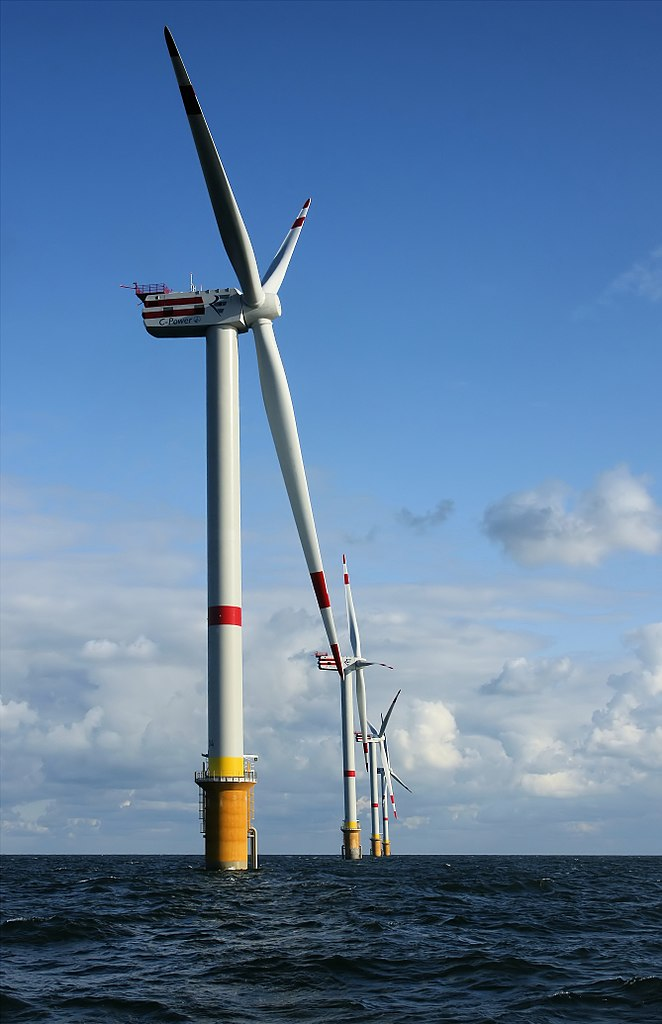
\includegraphics[width=0.7\textwidth]{img/Windmills_D1-D4.jpg}
				\caption*{Větrné elektrárny v Belgii.\footnote[frame]{Zdroj: \href{https://commons.wikimedia.org/wiki/File:Windmills_D1-D4_(Thornton_Bank).jpg}{Hans Hillewaert/Commons}}}
			\end{figure}
		\end{column}
	\end{columns}
}

\subsection{Lanthanoidy}
\frame{
	\frametitle{}
	\vfill
	\begin{itemize}
		\item Největší využití lanthanoidů je v katalýze.\footnote[frame]{\href{https://doi.org/10.1016/0022-5088(86)90254-7}{The role of the lanthanides in applied catalysis}}
		\item Více než 80~\% produkce lanthanoidů slouží pro přípravu katalyzátorů.
		\item Velká část se spotřebuje při rafinaci ropy.
		\item Využívají se také při zpracování syntetického plynu a přípravě složitějších organických sloučenin.\footnote[frame]{\href{https://doi.org/10.1021/es062888i}{Tracking Petroleum Refinery Emission Events Using Lanthanum and Lanthanides as Elemental Markers for PM2.5}}
		\item Jako katalyzátory mohou vystupovat přímo kovové lanthanoidy, jejich oxidy nebo složitější soli.
	\end{itemize}
	\begin{figure}
		\adjincludegraphics[width=1.05\textwidth]{img/Ln-catalysts.png}
	\end{figure}
	\vfill
}

\frame{
	\frametitle{}
	\vfill
	\begin{itemize}
		\item Slitina ceru, lanthanu, neodymu a dalších lanthanoidů se označuje jako \textit{Mischmetall}.
		\item Složení je přibližně 55~\% Ce, 25~\% La, 15--18~\% Nd a 5~\% Fe.
		\item Připravuje se elektrolýzou taveniny bezvodých chloridů.
		\item Je pyroforická.
		\item Využívá se jako kamínek do zapalovačů.
	\end{itemize}
	\begin{figure}
		\adjincludegraphics[width=0.5\textwidth]{img/Mischmetal.jpg}
		\caption*{Kousky mischmetallu.\footnote[frame]{Zdroj: \href{https://commons.wikimedia.org/wiki/File:Mischmetal.JPG}{Spypredator/Commons}}}
	\end{figure}
	\vfill
}

\frame{
	\frametitle{}
	\vfill
	\begin{columns}
		\begin{column}{.7\textwidth}
			\begin{itemize}
				\item Lanthanoidy se také využívají ke konstrukci permanentních magnetů.
				\item Ty jsou silnější než běžné permanentní magnety.
				\item Nejběžnější jsou neodymové magnety, ty jsou tvořen slitinou \ce{Nd2Fe14B} a samariové magnety \ce{SmCo5}.
				\item Vyrábějí se metodami práškové metalurgie.
				\item Využívají se např. v pevných discích, větrných turbínách, magnetických ložiscích.
				\item Halbachovy magnety -- přesně uspořádané pole magnetů, generuje silné pole na jedné straně a nulové pole na druhé.\footnote[frame]{\href{https://www.unimagnet.cz/clanek/506/magneticke-otazniky-21-co-je-halbachovo-pole-ci-magneticke-grippery/}{Co je Halbachovo pole či magnetické grippery?}}
			\end{itemize}
		\end{column}
		\begin{column}{.35\textwidth}
			\begin{figure}
				\adjincludegraphics[height=.6\textwidth,rotate=90]{img/Neodymag.jpg}
				\caption*{Neodymový magnet z pevného disku.\footnote[frame]{Zdroj: \href{https://commons.wikimedia.org/wiki/File:Mischmetal.JPG}{Spypredator/Commons}}}
			\end{figure}
		\end{column}
	\end{columns}
	\vfill
}

\frame{
	\frametitle{}
	\vfill
	\begin{columns}
		\begin{column}{.5\textwidth}
			\begin{figure}
				\adjincludegraphics[width=0.9\textwidth]{img/Halbach_array_by_Zureks.png}
				\caption*{Magnetické pole uvnitř Halbachova magnetu.\footnote[frame]{Zdroj: \href{https://commons.wikimedia.org/wiki/File:Halbach_array_by_Zureks.png}{Zureks/Commons}}}
			\end{figure}
		\end{column}
		\begin{column}{.5\textwidth}
			\begin{figure}
				\adjincludegraphics[width=0.9\textwidth]{img/Magritek-C10.jpg}
				\caption*{Stolní NMR spektrometr s Halbachovým magnetem.}
			\end{figure}
		\end{column}
	\end{columns}
	\vfill
}

\frame{
	\frametitle{}
	\vfill
	\textbf{Optoelektrické aplikace}
	\begin{itemize}
		\item Lanthanoidy jsou součástí pevnolátkových LASERů, zpravidla založených na granátu yttrito-hlinitém (\textbf{YAG}, \ce{Y3Al5O12}).\footnote[frame]{\href{http://www.lt.cz/e-learning/laser/princip-pevnolatkovych-nd-yag-laseru-1064-nm-infra-red}{Princip pevnolátkových Nd:YAG laserů}}
		\item Ve struktuře granátu jsou nahrazeny yttrité ionty za ionty lanthanoidů.
		\item Jeden z nejpoužívanějších je Nd:YAG LASER, který poskytuje záření o vlnové délce 1064~nm.\footnote[frame]{\href{https://circuitglobe.com/ndyag-laser.html}{Nd:YAG Laser}}
	\end{itemize}
	\begin{figure}
		\adjincludegraphics[height=0.32\textheight]{img/Powerlite_NdYAG.jpg}
		\caption*{Nd:YAG laser.\footnote[frame]{Zdroj: \href{https://commons.wikimedia.org/wiki/File:Powerlite_NdYAG.jpg}{Kkmurray/Commons}}}
	\end{figure}
	\vfill
}

\subsection{Aktinoidy}
\frame{
	\frametitle{}
	\vfill
	\begin{columns}
		\begin{column}{.75\textwidth}
		\begin{itemize}
			\item S aktinoidy se setkáváme v \textbf{jaderné energetice} a také u jaderných zbraní.
			\item Palivem pro současné jaderné reaktory je izotop $^{235}$U, jediný izotop uranu schopný štěpení.
			\item Pokud je jádro zasaženo neutronem o vhodné energii dojde k rozpadu na dvě lehčí jádra a uvolní se tři neutrony.
			\item Rozpad jednoho jádra $^{235}$U uvolní 202,5~MeV, to odpovídá 19,54~TJ.mol$^{-1}$.
			\item Pokud bychom nechali reakci neřízenou, dojde k řetězovému průběhu, který povede až k jadernému výbuchu.
			\item V jaderných reaktorech se využívá řídících a regulačních tyčí k snižování počtu neutronů v aktivní zóně.
		\end{itemize}
		\end{column}
		\begin{column}{.35\textwidth}
			\begin{figure}
				\adjincludegraphics[width=.9\textwidth]{img/Nuclear_fission.png}
				\caption*{Jaderné štěpení.\footnote[frame]{Zdroj: \href{https://commons.wikimedia.org/wiki/File:Nuclear_fission.svg}{Fastfission/Commons}}}
			\end{figure}
		\end{column}
	\end{columns}
	\vfill
}

\subsection{Jaderná energetika}
\frame{
	\frametitle{}
	\vfill
	\begin{itemize}
		\item[\textbf{1895}] Wilhel Conrad Röntgen objevil paprsky X
		\item[\textbf{1896}] Antoine Henri Becquerel objevil přírodní radioaktivitu studiem uranových solí
		\item[\textbf{1898}] Marie a Pierre Curieovi objevili polonium a radium
		\item[\textbf{1905}] Speciální teorie relativity, vztah mezi hmotou a energií: $\mathrm{E} = \mathrm{mc}^2$
		\item[\textbf{1926}] Geiger a Müller zkonstruovali detektor ionizujícího záření
		\item[\textbf{1932}] James Chadwick objevil neutron
		\item[\textbf{1934}] Irena a Frederic Joliot-Curieovi objevili umělou radioaktivitu
		\item[\textbf{1938}] Otto Hahn se spolupracovníky rozštěpil jádro uranu
		\item[\textbf{1942}] Projekt Manhattan; první jaderný reaktor
		\item[\textbf{1945}] Svržení atomových bomb na Hirošimu a Nagasaki
		\item[\textbf{1954}] První jaderná elektrárna (Obninsk, blízko Moskvy)
		\item[\textbf{1985}] Spuštěna jaderná elektrárna v Dukovanech
		\item[\textbf{1986}] Havárie v Černobylu
		\item[\textbf{2002}] Spuštěna jaderná elektrárna Temelín
		\item[\textbf{2011}] Fukušimská havárie
	\end{itemize}
	\vfill
}

\frame{
	\frametitle{}
	\vfill
	\begin{columns}
		\begin{column}{.7\textwidth}
			\textbf{Projekt Manhattan}
			\begin{itemize}
				\item Manhattan Engineering District -- vývoj atomové bomby během 2.~světové války.
				\item Přímo se na něm podílelo asi 225 000 lidí, nepřímo více než půl milionu.
				\item Jedna část projektu probíhala v nové zbudovaném městečku Oak Ridge v Tennessee, zde byl připravován obohacený $^{235}$U.
				\item V Los Alamos v Novém Mexiku byla vyvinuta atomová bomba.
				\item V Hanfordu ve Washingtonu byla optimalizována výroba plutonia.
				\item První atomová bomba byla testována v poušti v Novém Mexiku nedaleko města Alamogordo.
			\end{itemize}
		\end{column}
		\begin{column}{.35\textwidth}
			\begin{figure}
				\adjincludegraphics[height=0.55\textheight]{img/Los_Alamos_Primer_assembly_methods.png}
				\caption*{Různé možnosti dosažení nadkritického množství štěpného materiálu v jaderné bombě.\footnote[frame]{Zdroj: \href{https://commons.wikimedia.org/wiki/File:Los_Alamos_Primer_assembly_methods.png}{Robert Serber/Commons}}}
			\end{figure}
		\end{column}
	\end{columns}
	\vfill
}

\frame{
	\frametitle{}
	\vfill
	\textbf{Obohacený uran}
	\begin{itemize}
		\item Jako obohacený se označuje uran, který má vyšší koncentraci izotopu $^{235}$U než odpovídá přírodnímu uranu (0,71~\%).
		\item Separace izotopů $^{235}$U a $^{238}$U je obtížná, protože mají velmi podobné vlastnosti, využívá se rozdílu v jejich hmotnosti.
		\item Pro obohacení se využívá hlavně \textit{fluorid uranový}, \ce{UF6}, který snadno sublimuje.
		\item \ce{U + 2 ClF3 -> UF6 + Cl2}
		\item Fluorid lze poté hydrolyzovat na oxidy uranu.
		\item Fluor je monoizotopický, tím se zbavíme nutnosti řešit vyšší počet izotopologů\footnote[frame]{Izotopology -- látky, které se liší izotopickým složením} \ce{UF6}, skládá se pouze ze dvou: $^{235}$\ce{UF6} a $^{238}$\ce{UF6}.
		\item Metod obohacování je více, komerčně se využívají dvě:
		\begin{enumerate}
			\item Centrifugace
			\item Plynová difuze
			\item Elektromagnetická separace
		\end{enumerate}
	\end{itemize}
	\vfill
}

\frame{
	\frametitle{}
	\vfill
	\begin{columns}
		\begin{column}{.6\textwidth}
			\textbf{Centrifuga}
			\begin{itemize}
				\item Využívá se soustava velkého počtu válcových centrifug.\footnote[frame]{\href{https://fas.org/issues/nonproliferation-counterproliferation/nuclear-fuel-cycle/uranium-enrichment-gas-centrifuge-technology/centrifuge-works/}{How a Centrifuge Works}}
				\item Plyn se v rotujícím válci dělí podle hmotnosti, těžší částice jsou odstředivou silou tlačeny k vnější straně, lehčí se koncentrují uprostřed.
				\item Centrifugy mohou dosahovat až 50~000 otáček za sekundu.
				\item Zlepšení separačního poměru lze dosáhnout vytvořením teplotního gradientu v centrifuze.
			\end{itemize}
		\end{column}
		\begin{column}{.4\textwidth}
			\begin{figure}
				\adjincludegraphics[height=0.6\textheight]{img/Zippe-type_gas_centrifuge.png}
				\caption*{Centrifuga určená na obohacování uranu.\footnote[frame]{Zdroj: \href{https://commons.wikimedia.org/wiki/File:Zippe-type_gas_centrifuge.svg}{Fastfission/Commons}}}
			\end{figure}
		\end{column}
	\end{columns}
	\vfill
}

\frame{
	\frametitle{}
	\vfill
	\begin{figure}
		\adjincludegraphics[height=0.67\textheight]{img/Gas_centrifuge_cascade.jpg}
		\caption*{Soustava plynových centrifug.\footnote[frame]{Zdroj: \href{https://commons.wikimedia.org/wiki/File:Gas_centrifuge_cascade.jpg}{U.S. Department of Energy/Commons}}}
	\end{figure}
	\vfill
}

\frame{
	\frametitle{}
	\vfill
	\textbf{Plynová difuze}
	\begin{itemize}
		\item Plynný \ce{UF6} prochází přes polopropustnou membránu.\footnote[frame]{\href{https://www.centrusenergy.com/learn-more/uranium-enrichment/gaseous-diffusion/}{Gaseous Diffusion}}
		\item Těžší částice procházejí pomaleji než lehčí.
		\item $\frac{R_1}{R_2} = \sqrt{\frac{M_2}{M_1}} = \sqrt{\frac{352,041206}{349,0343448}} = 1,004298$
		\item $R_1, R_2$ -- rychlost efuze přes membránu
	\end{itemize}
	\begin{figure}
		\adjincludegraphics[height=0.4\textheight]{img/Gaseous_Diffusion.jpg}
		\caption*{Plynová difuze.\footnote[frame]{Zdroj: \href{https://commons.wikimedia.org/wiki/File:Gaseous_Diffusion_(44021367082)_(cropped).jpg}{Nuclear Regulatory Commission/Commons}}}
	\end{figure}
	\vfill
}

\frame{
	\frametitle{}
	\vfill
	\textbf{Elektromagnetická separace -- kalutron}
	\begin{itemize}
		\item Jde o hmotnostní spektrometr ve větším měřítku.\footnote[frame]{\href{https://doi.org/10.1016/S1044-0305(97)00123-2}{Preparative Scale Mass Spectrometry: A Brief History of the Calutron}}
		\item Plyn se ionizuje a dráha letících iontů je zakřivována působením magnetického pole.
		\item Poloměr zakřivení je úměrný poměru hmotnosti iontu a jeho náboje: $\frac{m}{z}$.
	\end{itemize}
	\begin{figure}
		\adjincludegraphics[height=0.38\textheight]{img/Calutron.jpg}
		\caption*{Kalutron.\footnote[frame]{Zdroj: \href{https://commons.wikimedia.org/wiki/File:Alpha_1_racetrack,_Uranium_235_electromagnetic_separation_plant,_Manhattan_Project,_Y-12_Oak_Ridge.jpg}{Leslie R. Groves/Commons}}}
	\end{figure}
	\vfill
}

\frame{
	\frametitle{}
	\vfill
	\textbf{První jaderná bomba -- Trinity}
	\begin{columns}
		\begin{column}{.75\textwidth}
			\begin{itemize}
				\item Jednalo se o plutoniovou bombu o síle 19 kilotun TNT.
				\item V době vývoje byl problém se získáním čistého plutonia, proto nebylo možné využít puškový model jaderné bomby.
				\item Místo toho byla bomba založena na implozním modelu, kde je kulové jádro tvořené plutoniem stlačeno \textit{současným} výbuchem nejaderných náloží.
				\item Tlak na jádro musí být ze všech stran stejný, aby došlo k dostatečnému zvýšení hustoty a tím k překročení tzv. \textit{kritického množství plutonia}. To je minimální množství nutné k iniciaci řetězové reakce.
				\item Odpálena byla 16. července 1945 v~poušti v~Novém Mexiku.
			\end{itemize}
		\end{column}
		\begin{column}{.35\textwidth}
			\begin{figure}
				\adjincludegraphics[height=0.5\textheight]{img/Fission_bomb_assembly_methods.png}\caption*{Puškový a implozní typ jaderné bomby.\footnote[frame]{Zdroj: \href{https://commons.wikimedia.org/wiki/File:Fission_bomb_assembly_methods.svg}{Fastfission/Commons}}}
			\end{figure}
		\end{column}
	\end{columns}
	\vfill
}

\frame{
	\frametitle{}
	\vfill
	\begin{figure}
		\adjincludegraphics[height=0.7\textheight]{img/Trinity_shot_color.jpg}
		\caption*{Výbuch Trinity, 16. 7. 1945.\footnote[frame]{Zdroj: \href{https://commons.wikimedia.org/wiki/File:Trinity_shot_color.jpg}{Jack W. Aeby/Commons}}}
	\end{figure}
	\vfill
}

\frame{
	\frametitle{}
	\vfill
	\textbf{Nagasaki a Hirošima}
	\begin{itemize}
		\item 6. srpna 1945 byla svržena uranová jaderná bomba \textit{Little Boy} na japonské město Hirošima. Na výrobu této bomby byl použit veškerý dostupný $^{235}$U.
		\item 9. srpna 1945 byla svržena plutoniová jaderná bomba \textit{Fat Man} na japonské město Nagasaki. Šlo o implozní typ bomby
	\end{itemize}

	\begin{figure}
		\adjincludegraphics[height=.5\textheight]{img/Gun-type_fission_weapon_en-labels_thin_lines.png}
		\caption*{Řez bombou Little Boy.\footnote[frame]{Zdroj: \href{https://en.wikipedia.org/wiki/File:Gun-type_fission_weapon_en-labels_thin_lines.svg}{FastFission/Commons}}}
	\end{figure}
	\vfill
}

\frame{
	\frametitle{}
	\vfill
	\begin{columns}
		\begin{column}{.5\textwidth}
			\begin{figure}
				\adjincludegraphics[height=.4\textheight]{img/Little_boy.jpg}
				\caption*{Little Boy.\footnote[frame]{Zdroj: \href{https://commons.wikimedia.org/wiki/File:Little_boy.jpg}{U.S. National Archives/Commons}}}
			\end{figure}
		\end{column}
		\begin{column}{.5\textwidth}
			\begin{figure}
				\adjincludegraphics[height=.4\textheight]{img/Fat_man.jpg}
				\caption*{Fat man.\footnote[frame]{Zdroj: \href{https://commons.wikimedia.org/wiki/File:Fat_man.jpg}{U.S. Department of Defense/Commons}}}
			\end{figure}
		\end{column}
	\end{columns}
	\vfill
}

\frame{
	\frametitle{}
	\vfill
	\begin{figure}
		\adjincludegraphics[height=0.7\textheight]{img/Nagasaki_1945_-_Before_and_after.jpg}
		\caption*{Nagasaki před a po bombardování.\footnote[frame]{Zdroj: \href{https://commons.wikimedia.org/wiki/File:Nagasaki_1945_-_Before_and_after.jpg}{U.S. National Archives/Commons}}}
	\end{figure}
	\vfill
}

\frame{
	\frametitle{}
	\vfill
	\begin{columns}
		\begin{column}{.6\textwidth}
			\begin{itemize}
				\item Podle odhadů zemřelo bezprostředně po bombardování v Hirošimě přibližně 150~000 lidí a v Nagasaki téměř 80~000 lidí.
				\item Bombardování vedlo ke kapitulaci Japonska. USA měly připravené další čtyři jaderné bomby, které už ale nebyly použity.
			\end{itemize}
			\begin{figure}
				\adjincludegraphics[height=0.25\textheight]{img/Hiroshima-pref-prom-hall-04.jpg}
				\caption*{Hiroshima.\footnote[frame]{Zdroj: \href{https://commons.wikimedia.org/wiki/File:Hiroshima-pref-prom-hall-04.jpg}{Michael Reeve/Commons}}}
			\end{figure}
		\end{column}
		\begin{column}{.4\textwidth}
			\begin{figure}
				\adjincludegraphics[height=0.55\textheight]{img/Atomic_cloud_over_Hiroshima.jpg}
				\caption*{Atomový hřib nad Hirošimou.\footnote[frame]{Zdroj: \href{https://commons.wikimedia.org/wiki/File:Atomic_cloud_over_Hiroshima.jpg}{George R. Caron/Commons}}}
			\end{figure}
		\end{column}
	\end{columns}
	\vfill
}

\frame{
	\frametitle{}
	\vfill
	\textbf{Jaderné elektrárny}
	\begin{itemize}
		\item Elektrárna využívající vazebnou energii atomových jader k výrobě elektrické energie.
		\item Jako palivo se zpravidla využívá obohacený uran, který obsahuje 2--5~\% izotopu $^{235}$U.
		\item Podzemní zásoby uranu jsou dostatečné na více než 250 let.\footnote[frame]{\href{https://www.osel.cz/3778-bude-dost-surovin-pro-jadernou-energetiku.html}{Bude dost surovin pro jadernou energetiku?}}
		\item Podstatně více uranu je uloženo v mořské vodě, odhaduje se až $10^{10}$~tun, ale koncentrace je velmi nízká, zhruba $10^{-7}$--$10^{-9}$~g.l$^{-1}$
		\item Jaderná elektrárna je v principu parní elektrárna.
		\item Jaderný reaktor generuje teplo pro ohřev vody na páru a ta pohání turbíny, které generují elektrický proud.
		\item Na rozdíl od bomb je nutné se vyvarovat řetězovému průběhu jaderné reakce, proto reaktory obsahují prvky, které snižují počet volných neutronů.
	\end{itemize}
	\vfill
}

\frame{
	\frametitle{}
	\vfill
	\begin{figure}
		\adjincludegraphics[height=0.7\textheight]{img/Nuclear_power_plant-pressurized_water_reactor-PWR.png}
		\caption*{Schéma jaderné elektrárny.\footnote[frame]{Zdroj: \href{https://commons.wikimedia.org/wiki/File:Nuclear_power_plant-pressurized_water_reactor-PWR.png}{Steffen Kuntoff/Commons}}}
	\end{figure}
	\vfill
}

\frame{
	\frametitle{}
	\vfill
	\begin{itemize}
		\item Existuje mnoho typů jaderných reaktorů.
		\item \textit{Pomalé reaktory} vyžadují moderátor (grafit nebo vodu) pro zpomalení neutronů. Jako palivo využívají tyče z uranu nebo \ce{UO2}.
		\item \textit{Rychlé reaktory} moderátor nevyžadují. Jako palivo využívají \ce{^{239}PuO2}.
		\item V České republice jsou v provozu dvě jaderné elektrárny.
		\item \textit{JE Dukovany} se začala budovat v roce 1978 a spouštěna byla v roce 1985-1987.\footnote[frame]{\href{https://oenergetice.cz/jaderne-elektrarny/jaderna-elektrarna-dukovany}{Jaderná elektrárna Dukovany je v provozu od roku 1985}}
		\item Je umístěna 30 km od Třebíče.
		\item V současnosti generuje 14~TWh ročně.
		\item Má čtyři tlakovodní reaktory VVER 440/213, palivem je uran obohacený na 4,25~\% $^{235}$U. V reaktoru je 42 tun paliva.
		\item Reaktory jsou uloženy v kontejnmentu, který v případě havárie zajistí ochlazení páry a snížení tlaku.
	\end{itemize}
	\vfill
}

\frame{
	\frametitle{}
	\vfill
	\begin{figure}
		\adjincludegraphics[height=0.7\textheight]{img/Nuclear.power.plant.Dukovany.jpg}
		\caption*{Jaderná elektrárna Dukovany.\footnote[frame]{Zdroj: \href{https://commons.wikimedia.org/wiki/File:Nuclear.power.plant.Dukovany.jpg}{Petr Adamek/Commons}}}
	\end{figure}
	\vfill
}

\frame{
	\frametitle{}
	\vfill
	\begin{columns}
		\begin{column}{.65\textwidth}
			\begin{itemize}
				\item JE Temelín se začala stavět v roce 1987 v Jihočeském kraji, 25~km od Českých Budějovic.
				\item Spuštěna byla 10. června 2002. Ročně produkuje více než 15~TWh.
				\item Z původně plánovaných čtyř bloků byly postaveny jen dva, každý je osazen tlakovodním reaktorem VVER 1000/V-320.
				\item Reaktory jsou také uloženy v kontejnmentu. Kontejnment má výšku 38~m, průměr 45~m a tloušťku stěn 1,2~m. Kontejnmenty jsou podtlakované, aby se zabránilo úniku radioaktivity ven.
				\item Palivem je \ce{UO2} obohacený na 4,25~\% $^{235}$U. V každém reaktoru je 92 tun paliva.
			\end{itemize}
		\end{column}
		\begin{column}{.4\textwidth}
			\begin{figure}
				\adjincludegraphics[height=0.65\textheight]{img/Containment_Building.jpg}
				\caption*{Kontejnment.\footnote[frame]{Zdroj: \href{https://commons.wikimedia.org/wiki/File:Containment_Building.jpg}{NRC/Commons}}}
			\end{figure}
		\end{column}
	\end{columns}
	\vfill
}

\frame{
	\frametitle{}
	\vfill
	\begin{figure}
		\adjincludegraphics[height=0.7\textheight]{img/JETE3.jpg}
		\caption*{Jaderná elektrárna Temelín.\footnote[frame]{Zdroj: \href{https://commons.wikimedia.org/wiki/File:JETE3.JPG}{Japo/Commons}}}
	\end{figure}
	\vfill
}

\frame{
	\frametitle{}
	\vfill
	\textbf{PUREX -- \textbf{P}lutonium \textbf{U}ranium \textbf{R}eduction \textbf{Ex}traction}
	\begin{itemize}
		\item Technologický proces vyvinutý během projektu Manhattan k získávání plutonia a uranu z vyhořelého jaderného paliva.\footnote[frame]{\href{http://www.igcar.gov.in/rpg/articles/Ramanujam - Intro to reporcessing.pdf}{An Introduction to the Purex Process}}
		\item Je založen na rozdílných redoxních vlastnostech uranu, neptunia a plutonia a rozdílu v extrakci sloučenin těchto kovů do roztoku TBP v kerosenu.
		\item Materiál se rozpustí v kyselině dusičné, čímž získáme směs iontů \ce{UO$_2^{2+}$}, \ce{NpO$_2^{+}$} a \ce{Pu(NO3)$_6^{2-}$}.\footnote[frame]{HÁLA, Jiří. \textit{Radioaktivní izotopy}. Tišnov: Sursum, 2013. ISBN 978-80-7323-248-1.}
		\item Přídavkem dusitanu dojde k oxidaci neptunia na \ce{NpO$_2^{2+}$} a všechny tři ionty jsou extrahovány pomocí roztoku tributylfosfátu v kerosinu.
	\end{itemize}
	\vfill
}

\frame{
	\frametitle{}
	\vfill
	\begin{figure}
		\adjincludegraphics[height=0.9\textheight,rotate=90]{img/Extracteduraniumcomplex.png}
		\caption*{Struktura komplexu uranu v extraktu.\footnote[frame]{Zdroj: \href{https://commons.wikimedia.org/wiki/File:Extracteduraniumcomplex.png}{Cadmium/Commons}}}
	\end{figure}
	\vfill
}

\frame{
	\frametitle{}
	\vfill
	\begin{itemize}
		\item Přídavkem dusitanu dojde k oxidaci neptunia na \ce{NpO$_2^{2+}$} a všechny tři ionty jsou extrahovány pomocí roztoku tributylfosfátu v kerosinu.
		\item Extrakt obsahuje pouze ionty uranu, neptunia a plutonia. Železnatou solí se zredukuje plutonium a neptunium na \ce{Pu^{3+}} a \ce{Np^{4+}}. V tomto kroku dojde k přechodu plutonité soli do vodného prostředí a je dále zpracováváno, zatímco uran a neptunium zůstávají v organické fázi.
		\item Dalším krokem je převedením zbylých iontů do vodného roztoku a extrakce 1--2~M kyselinou dusičnou, čímž se oddělí uran od neptunia.
		\item V současnosti se tato metoda využívá ve Francii, Velké Británii, Japonsku a Rusku k přepracování jaderného paliva.
		\item Lze jej použít i k přípravě tzv. \textit{MOX paliva} (\textit{M}ixed \textit{OX}ide fuel: \ce{PuO2} a \ce{UO2}), které je dnes už možné využívat v reaktorech. Tím se separace zjednoduší.
	\end{itemize}
	\vfill
}

\frame{
	\frametitle{}
	\vfill
	\begin{table}
		\begin{tabular}{|l|l|}
			\hline
			\textbf{Název procesu} & \textbf{Separované kovy} \\\hline
			\ce{BiPO4} proces & Pu \\\hline
			Fluorido--acetátový & Pu \\\hline
			REDOX & U, Pu \\\hline
			TRIGLY & U, Pu \\\hline
			BUTEX & U, Pu \\\hline
			PUREX & U, Np, Pu \\\hline
			THOREX & Th, U \\\hline
			Pyrometalurgické zpracování & U, Pu \\\hline
			Pyrochemické zpracování & U, Pu \\\hline
			Fluoridový proces & U, Pu \\\hline
		\end{tabular}
		\caption*{Významné separační technologie.\footnote[frame]{\href{https://world-nuclear.org/information-library/nuclear-fuel-cycle/fuel-recycling/processing-of-used-nuclear-fuel.aspx}{Processing of Used Nuclear Fuel}}}
	\end{table}
	\vfill
}

\frame{
	\frametitle{}
	\vfill
	\begin{figure}
		\adjincludegraphics[height=0.7\textheight]{img/Purexraffinatecomp.png}
		\caption*{Zastoupení prvků v extraktu.\footnote[frame]{Zdroj: \href{https://commons.wikimedia.org/wiki/File:Purexraffinatecomp.png}{Cadmium/Commons}}}
	\end{figure}
	\vfill
}

\frame{
	\frametitle{}
	\vfill
	\begin{figure}
		\adjincludegraphics[height=0.7\textheight]{img/Uranium_Reprocessing.jpg}
		\caption*{Schéma procesu PUREX.\footnote[frame]{Zdroj: \href{https://commons.wikimedia.org/wiki/File:Uranium_Reprocessing.jpg}{Koonzybear/Commons}}}
	\end{figure}
	\vfill
}

\frame{
	\frametitle{}
	\vfill
	\textbf{Přírodní reaktory}
	\begin{itemize}
		\item Přírodní jaderný reaktor v Oklo, ve státě Gabon na západním pobřeží Afriky.\footnote[frame]{\href{http://webmineral.com/data/Thortveitite.shtml}{Meet Oklo, the Earth’s Two-billion-year-old only Known Natural Nuclear Reactor}}
		\item Reaktor byl objeven analýzou izotopického složení uranových rud.
		\item Přírodní uran dnes obsahuje 0,7202~\% izotopu $^{235}$U, díky dlouhému poločasu rozpadu je toto složení stabilní.
		\item Uranová ruda z oblasti Oklo, ale ukázala zastoupení izotopu $^{235}$U jen 0,7171~\%, což je velmi významný rozdíl.
		\item Další zkoumání oblasti ukázalo, že došlo k samovolné iniciaci jaderné reakce, díky povětrnostním vlivům se nashromáždilo nadkritické množství.
		\item V té době bylo také vyšší zastoupení izotopu $^{235}$U -- okolo 3~\%.
	\end{itemize}
	\vfill
}

\frame{
	\frametitle{}
	\vfill
	\begin{figure}
		\adjincludegraphics[height=0.65\textheight]{img/Gabon_Geology_Oklo.png}
		\caption*{Schéma přírodního reaktoru v Oklo. 1 - jaderný reaktor; 2 - pískovec; 3 - uranová ruda; 4 - žula\footnote[frame]{\href{https://commons.wikimedia.org/wiki/File:Gabon_Geology_Oklo.svg}{Zdroj: MesserWoland/Commons}}}
	\end{figure}
	\vfill
}

\frame{
	\frametitle{}
	\vfill
	\begin{itemize}
		\item Jako moderátor neutronů sloužila voda v jílových horninách. Fluktuace množství vody daná teplem jaderné reakce způsobovala pulzních chod reaktoru.\footnote[frame]{\href{http://www-ucjf.troja.mff.cuni.cz/cejnar/publikace/Oklo.htm}{Oklo – jaderné reaktory z pravěku}}
		\begin{itemize}
			\item Zvýšením teploty dochází k přeměně vody na páru, která hůře zpomaluje neutrony.
			\item Tím dojde ke zpomalení jaderné reakce a následnému snížení teploty.
			\item To umožní opětovné zaplavení aktivní zóny reaktoru vodou.
		\end{itemize}
		\item Velký vliv také měly horniny obsahující bór a prvky vzácných zemin, které dokáží absorbovat neutrony.
		\item Analýzou oblasti bylo prokázáno, že byl reaktor v provozu před dvěma miliardami let, doba provozu je odhadována na 150 tisíc let při výkonu asi 100~kW na zónu. Nalezeno bylo 16 reaktorových zón.
		\item Dnes už jaderná reakce v oblasti neprobíhá a ani nelze očekávat, že by došlo k dalšímu samovolnému spuštění. Důvodem je snížení přirozené koncentrace izotopu $^{235}$U radioaktivním rozpadem.
	\end{itemize}
	\vfill
}

\section{Sloučeniny}
\subsection{Hydridy}
\frame{
	\frametitle{}
	\vfill
	\begin{itemize}
		\item Reakcí lanthanoidů s vodíkem za teploty nad 300~$^\circ$C vznikají černé hydridy \ce{LnH2}.\footnote[frame]{\href{https://www.radiochemistry.org/periodictable/la_series/L11.html}{Lanthanide Hydrides}}
		\item Mají fluoritovou strukturu a kubickou, plošně centrovanou mřížku.\footnote[frame]{\href{https://doi.org/10.1021/j100807a033}{Crystal structures of some lanthanide hydrides}}
		\item Za vyššího tlaku se obsah vodíku zvyšuje, vodík se dostává do intersticiálních poloh v krystalové mřížce.
		\item Zvyšováním tlaku se lze dostat až k limitní stechiometrii \ce{LnH3}.
		\item Výjimkou jsou Eu a Yb, které preferují složení \ce{LnH2}.
	\end{itemize}
	\vfill
}

\frame{
	\frametitle{}
	\vfill
	\begin{columns}
		\begin{column}{.5\textwidth}
			\begin{figure}
				\adjincludegraphics[height=0.45\textheight]{img/Calcium-fluoride-3D-ionic.png}
				\caption*{Struktura fluoritu.\footnote[frame]{Zdroj: \href{https://commons.wikimedia.org/wiki/File:Calcium-fluoride-3D-ionic.png}{Benjah-bmm27/Commons}}}
			\end{figure}
		\end{column}
		\begin{column}{.5\textwidth}
			\begin{figure}
				\adjincludegraphics[height=0.45\textheight]{img/CaF2_polyhedra.png}
				\caption*{Koordinační polyedry ve fluoritové struktuře.\footnote[frame]{Zdroj: \href{https://commons.wikimedia.org/wiki/File:CaF2_polyhedra.png}{Solid State/Commons}}}
			\end{figure}
		\end{column}
	\end{columns}
	\vfill
}

\frame{
	\frametitle{}
	\vfill
	\begin{columns}
		\begin{column}{.5\textwidth}
			\begin{itemize}
				\item Dekahydrid lanthanu, \ce{LaH10}.\footnote[frame]{\href{https://www.acs.org/content/acs/en/molecule-of-the-week/archive/l/lanthanum-decahydride.html}{Lanthanum decahydride}}
				\item Lze jej připravit stlačením lanthanu a vodíku na tlak 200~GPa v diamantové kovadlině.\footnote[frame]{\href{https://doi.org/10.1038/s41586-019-1201-8}{Superconductivity at 250 K in lanthanum hydride under high pressures}}
				\item Je to supravodič s rekordní kritickou teplotou $-$13~$^\circ$C, bohužel je stabilní jen za extrémně vysokých tlaků.\footnote[frame]{\href{https://arxiv.org/ftp/arxiv/papers/1810/1810.01113.pdf}{Superconductivity of \ce{LaH10} and \ce{LaH16} polyhydrides}}
			\end{itemize}
		\end{column}
		\begin{column}{.5\textwidth}
			\begin{figure}
				\adjincludegraphics[width=.8\textwidth]{img/LaH10.png}
			\end{figure}
		\end{column}
	\end{columns}
	\vfill
}

\frame{
	\frametitle{}
	\vfill
	\begin{figure}
		\adjincludegraphics[height=.7\textheight]{img/Diamond_Anvil_Cell_-_Cross_Section.png}
		\caption*{Řez diamantovou kovadlinou.\footnote[frame]{Zdroj: \href{https://commons.wikimedia.org/wiki/File:Diamond_Anvil_Cell_-_Cross_Section.svg}{Tobias1984/Commons}}}
	\end{figure}
	\vfill
}

\subsection{Oxidy a hydroxidy}
\frame{
	\frametitle{}
	\vfill
	\begin{itemize}
		\item Oxidy \ce{Sc2O3} a \ce{Y2O3} krystalují v kubické soustavě, kovy mají koordinační číslo šest.
		\item \ce{La2O3} má stejnou strukturu, ale až za vyšší teploty. Za laboratorní teploty má lanthan koordinační číslo sedm.
		\item \ce{La2O3} reaguje prudce s vodou.
		\item \ce{La2O3 + 3 H2O -> 2 La(OH)3}
		\item Hydroxid skanditý je spíše hydratovaný oxid, v nadbytku NaOH se rozpouští:
		\item \ce{Sc(OH)3 + 3 NaOH -> Na3[Sc(OH)6]}
		\item Oxidy \ce{Ln2O3} jsou všechny dobře charakterizované a silně bazické. Bazicitou jsou podobné oxidům 2. skupiny.
		\item Ve vodě se nerozpouštějí, ale hydratují se za vzniku příslušných hydroxidů.
		\item V kyselinách se rozpouštějí za tvorby aqua komplexů.
	\end{itemize}
	\vfill
}

\frame{
	\frametitle{}
	\vfill
	\begin{itemize}
		\item U oxidů \ce{Ln2O3} známe tři strukturní typy:
		\item \textit{Typ A} - skládá se z jednotek \ce{LnO7}, ty jsou tvořeny oktaedrem se sedmým atomem kyslíku nad jednou z jeho stran. Jde především o oxidy lehčích lanthanoidů.
		\item \textit{Typ B} - také se skládá z jednotek \ce{LnO7}, ale  geometrii trigonálního prizmatu doplněného o jeden vrchol. Tento strukturní typ preferují lanthanoidy střední hmotnosti.
		\item \textit{Typ C} - můžeme odvodit ze struktury fluoritu odstraněním čtvrtiny aniontů. Koordinační číslo tak klesne na 6. Tento strukturní typ preferují lanthanoidy střední a vyšší hmotnosti.
	\end{itemize}
	\vfill
}

\frame{
	\frametitle{}
	\vfill
	\begin{columns}
		\begin{column}{.35\textwidth}
			\begin{figure}
				\adjincludegraphics[width=\textwidth]{img/A-Nd2O3.png}
				\caption*{Oktaedr doplněný o jeden vrchol.\footnote[frame]{Zdroj: \href{https://commons.wikimedia.org/wiki/File:A-Nd2O3-xtal-Nd-coordination-3D-bs-17.png}{Ben Mills/Commons}}}
			\end{figure}
		\end{column}

		\begin{column}{.35\textwidth}
			\begin{figure}
				\adjincludegraphics[width=\textwidth]{img/MonocappTrigPrismCapSupps.png}
				\caption*{Trigonální prisma doplněné o jeden vrchol.\footnote[frame]{Zdroj: \href{https://commons.wikimedia.org/wiki/File:MonocappTrigPrismCapSupps.png}{J3D3/Commons}}}
			\end{figure}
		\end{column}

		\begin{column}{.4\textwidth}
			\begin{figure}
				\adjincludegraphics[width=\textwidth]{img/CaF2_polyhedra.png}
				\caption*{Struktura fluoritu.\footnote[frame]{Zdroj: \href{https://commons.wikimedia.org/wiki/File:CaF2_polyhedra.png}{Solid State/Commons}}}
			\end{figure}
		\end{column}
	\end{columns}
	\vfill
}

\frame{
	\frametitle{}
	\vfill
	\begin{itemize}
		\item Oxidy aktinoidů jsou vysoce tepelně odolné.
		\item Oxid uranový, \ce{UO3}, lze připravit jako oranžovou modifikaci $\gamma$-\ce{UO3} tepelným rozkladem dusičnanu uranylu, \ce{UO2(NO3)2.6H2O}.
		\item Redukcí vodíkem získáme \ce{UO2}.
		\item Nejstabilnějším oxidem uranu je zelený až černý \ce{U3O8}, který je možné připravit zahříváním jiných oxidů uranu na teplotu \mbox{800--900~$^\circ$C}.
		\item \ce{U3O8} můžeme popsat jako oxid uraničito-diuranový \ce{UO2.2UO3}.
		\item Jeho struktura sestává z pentagonálních bipyramid \ce{UO7}.
	\end{itemize}
	\begin{figure}
		\adjincludegraphics[height=.27\textheight]{img/Triuranium_octoxide.jpg}
		\caption*{\ce{U3O8}.\footnote[frame]{Zdroj: \href{https://commons.wikimedia.org/wiki/File:Triuranium_octoxide.JPG}{Leiem/Commons}}}
	\end{figure}
	\vfill
}

\frame{
	\frametitle{}
	\vfill
	\begin{figure}
		\adjincludegraphics[width=.8\textwidth]{img/Kristallstruktur_Triuranoctoxid.png}
		\caption*{Struktura \ce{U3O8}.\footnote[frame]{Zdroj: \href{https://commons.wikimedia.org/wiki/File:Kristallstruktur_Triuranoctoxid.png}{Orci/Commons}}}
	\end{figure}
	\vfill
}

\frame{
	\frametitle{}
	\vfill
	\begin{itemize}
		\item Kalcinací s oxidy alkalických kovů vznikají směsné oxidy:
		\item \ce{10 Li2O + 2 PuO2 ->[O2, 420 $^\circ$C] 2 Li5PuO6}
		\item Podle poměru výchozích látek lze připravit mnoho různých stechiometrií:
		\begin{itemize}
			\item \ce{M2U2O7} -- diuranany
			\item \ce{M2UO4}, \ce{M4UO5}, \ce{M6UO6} -- uranany
			\item \ce{MAnO3}
			\item \ce{M3AnO4}
			\item \ce{M5AnO5}
		\end{itemize}
	\item Tyto sloučeniny obsahují oktaedrický ion \ce{AnO6}.
	\item Směsné oxidy uranu v oxidačním čísle V obsahují skutečně \ce{U^V}, nikoliv směs \ce{U^{IV}} a \ce{U^{VI}}.
	\item Oxidy \ce{BaAn^{IV}O3} (An = Th--Am) se připravují z \ce{AnO2}, v případě Pa a U v inertní atmosféře, v případě Am v atmosféře kyslíku.
	\end{itemize}
	\vfill
}

\frame{
	\frametitle{}
	\vfill
	\begin{columns}
		\begin{column}{.7\textwidth}
			\begin{itemize}
				\item \textit{Peroxid uranylu}, \ce{UO4}, \ce{(UO2)O2}, je žlutá pevná látka.
				\item Je jedním z meziproduktů při obohacování uranu.
				\item V přírodě se vyskytuje jako minerál studtit (\ce{UO4.4H2O})\footnote[frame]{\href{http://webmineral.com/data/Studtite.shtml}{Studtite Mineral Data}} nebo metastudtit (\ce{UO4.2H2O})\footnote[frame]{\href{http://webmineral.com/data/Metastudtite.shtml}{Metastudtite Mineral Data}}.
				\item Jedná se o jediné minerály obsahující peroxidový anion.\footnote[frame]{\href{https://dx.doi.org/10.1126/science.1090259}{Stability of Peroxide-Containing Uranyl Minerals}}
			\end{itemize}
		\end{column}
		\begin{column}{.3\textwidth}
			\begin{figure}
				\adjincludegraphics[height=0.37\textheight]{img/Uranylperoxide_Powder.jpg}
				\caption*{Peroxid uranylu.\footnote[frame]{Zdroj: \href{https://commons.wikimedia.org/wiki/File:Uranylperoxide_Powder.jpg}{Chemolunatic/Commons}}}
			\end{figure}
		\end{column}
	\end{columns}
	\vfill
}

\subsection{Halogenidy}
\frame{
	\frametitle{}
	\vfill
	\begin{itemize}
		\item \textbf{Skandium}
		\item \textit{Fluorid skanditý} je málo rozpustný ve vodě, ale rozpouští se v přítomnosti fluoridů za tvorby oktaedrických aniontů \ce{ScF$_6^{3-}$}.\footnote[frame]{\href{https://doi.org/10.1134/S1070427211080040}{Preparation and examination of the properties of complex scandium fluorides}}
		\item \ce{ScF3 + 3 KF ->[H2O] K3[ScF6]}
		\item \textit{Chlorid skanditý} a další halogenidy jsou dobře rozpustné ve vodě:
		\item \ce{ScCl3 + 6 H2O -> [Sc(H2O)6]Cl3}
		\item Připravují se přímou reakcí kovu s halogenem.
		\item \ce{2 Sc + 3 Cl2 -> 2 ScCl3}
		\item \ce{2 Sc + 3 Br2 -> 2 ScBr3}
		\item \ce{2 Sc + 3 I2 -> 2 ScI3}
	\end{itemize}
	\vfill
}

\frame{
	\frametitle{}
	\vfill
	\begin{itemize}
		\item \textbf{Yttrium}
		\item \textit{Fluorid yttritý}, \ce{YF3}, můžeme připravit reakcí yttria nebo hydroxidu yttritého s kyselinou fluorovodíkovou.
		\item V přírodě se vyskytuje jako minerál waimirit-(Y).\footnote[frame]{\href{https://www.mindat.org/min-46049.html}{Waimirite-(Y)}}
		\item \textit{Chlorid yttritý}, \ce{YCl3}, vytváří při přípravě z roztoku HCl hexahydrát.
		\item \ce{Y2O3 + 6 HCl + 9 H2O -> 2 YCl3.6H2O}
		\item Hydrát nelze termicky vysušit, dochází ke vzniku oxidu-chloridu \ce{YOCl}.
		\item Struktura je tvořena oktaedry \ce{YCl6} propojenými vrcholy.
		\item \textit{Bromid yttritý}, \ce{YBr3}, je bezbarvá, hygroskopická látka.
		\item Bezvodý lze připravit reakcí oxidu s bromidem amonným.\footnote[frame]{\href{https://doi.org/10.1016/0022-5088(87)90372-9}{The ammonium-bromide route to anhydrous rare earth bromides \ce{MBr3}}}
		\item \ce{Y2O3 + 6 NH4Br + 6 HBr -> 2 (NH4)3YBr6 + 3 H2O}
		\item \ce{(NH4)3YBr6 ->[400 $^\circ$C] YBr3 + 3 NH4Br}
	\end{itemize}
	\vfill
}

\frame{
	\frametitle{}
	\vfill
	\begin{columns}
		\begin{column}{.7\textwidth}
			\begin{itemize}
				\item \textbf{Lanthan}
				\item \textit{Fluorid lanthanitý}, \ce{LaF3}, je bílá pevná látka.
				\item Můžeme jej připravit reakcí yttria nebo hydroxidu yttritého s kyselinou fluorovodíkovou.
				\item Má strukturu trigionálního prizmatu doplněného o dva vrcholy (\textit{Bicapped Trigonal Prisma}).
				\item Koordinační číslo \ce{La^{3+}} je 11.
				\item V přírodě se vyskytuje jako velmi vzácný minerál fluocerit-(La).\footnote[frame]{\href{https://www.mindat.org/min-1568.html}{Fluocerite-(La)}}
			\end{itemize}
		\end{column}
		\begin{column}{.3\textwidth}
			\begin{figure}
				\adjincludegraphics[height=0.33\textheight]{img/LaF3_structure.png}
				\caption*{Struktura \ce{LaF3}.\footnote[frame]{Zdroj: \href{https://commons.wikimedia.org/wiki/File:LaF3_structure.svg}{Begoon/Commons}}}
			\end{figure}
		\end{column}
	\end{columns}
	\vfill
}

\frame{
	\frametitle{}
	\vfill
	\begin{itemize}
		\item \textit{Chlorid lanthanitý}, \ce{LaCl3}, je bílá pevná látka.
		\item Lze jej připravit přímou reakcí z prvků, ale běžnější je reakce oxidu se salmiakem:
		\item \ce{La2O3 + 6 NH4Cl ->[250 $^\circ$C] 2 LaCl3 + 6 NH3 + 2 H2O}
		\item Má vlastnosti Lewisovy kyseliny, čehož se využívá v katalýze.\footnote[frame]{\href{https://doi.org/10.3998/ark.5550190.0008.d23}{Lanthanum trichloride: an efficient Lewis acid catalyst for chemo and regioselective enamination of $\beta$-dicarbonyl compounds}}
		\item \textit{Bromid lanthanitý}, \ce{LaBr3}, je bílá, silně hygroskopická pevná látka.
		\item Vytváří několik hydrátů.
		\item Krystaly dopované cerem, \ce{LaBr3$:$Ce}, se využívají pro konstrukci scintilačních detektorů.\footnote[frame]{\href{https://doi.org/10.3998/ark.5550190.0008.d23}{High-energy-resolution scintillator: \ce{Ce^{3+}} activated \ce{LaBr3}}}
	\end{itemize}
	\vfill
}

\frame{
	\frametitle{}
	\vfill
	\begin{itemize}
		\item \textbf{Lanthanoidy}
		\item Lanthanoidy vytvářejí tři řady halogenidů: \ce{LnX4}, \ce{LnX3} a~\ce{LnX2} a také nižší halogenidy \ce{LnCl_x} (x = 1--1,714).
		\item \ce{LnF4} známe jen od Ce a Pr. Ostatní jsou termicky nestabilní.
		\item \ce{LnX3} jsou známy všechny.
		\item Dihalogenidy se získávají redukcí \ce{LnX3} kovovým lanthanoidem:
		\item \ce{2 LnX3 + Ln -> 3 LnX2}
		\item Dijodidy lze připravit reakcí kovu s 1,2-dijodethanem:
		\item \ce{Ln + ICH2CH2I -> LnI2 + CH2=CH2}
	\end{itemize}
	\vfill
}

\frame{
	\frametitle{}
	\vfill
	\begin{itemize}
		\item \textbf{Aktinoidy}
		\item Hexahalogenidy a pentahalogenidy aktinoidů jsou známé pouze od U, Np a Pu.
		\item Hexafluoridy se chovají podobně jako anhydridy, reakcí s vodou vzniká \ce{AnO2F2}.
		\item Tetrafluoridy známe až po \ce{CfF4}, všechny jsou nerozpustné ve vodě.
		\item Tetrachloridy se připravují chlorací oxidů \ce{AnO2} pomocí \ce{CCl4}, jsou dobře rozpustné ve vodě, stejně jako tetrabromidy a tetrajodidy.
	\end{itemize}
	\vfill
}

\subsection{Dusičnany}
\frame{
	\frametitle{}
	\vfill
	\begin{itemize}
		\item Dusičnany lanthanoidů, \ce{Ln(NO3)3}, jsou bílé pevné látky, mimo zeleného \ce{Pr(NO3)3} a fialového \ce{Nd(NO3)3}.
	\end{itemize}
	\begin{figure}
		\adjincludegraphics[width=\textwidth]{img/Lanthanide_nitrates.png}
		\caption*{Dusičnany \ce{Ln(NO3)3}: La, Ce, Pr, Nd, Sm, Eu, Gd, Tb, Dy, Ho, Er, Tm, Yb, Lu.\footnote[frame]{Zdroj: \href{https://commons.wikimedia.org/wiki/File:Lanthanide_nitrates.png}{Leiem/Commons}}}
	\end{figure}
	\vfill
}

\subsection{Komplexní sloučeniny}
\frame{
	\frametitle{}
	\vfill
	\begin{itemize}
		\item \textbf{Sc, Y, La}
		\item Komplexní sloučeniny těchto prvků mají nejčastěji koordinační číslo šest: \ce{[ScF6]^{3-}}, \ce{[Sc(bipy)3]^{3+}}.
		\item Vyššího koordinačního čísla (až 12) dosahují pouze komplexy s malými chelátovými ligandy -- \ce{SO$_4^{2-}$} a \ce{NO$_3^-$}.
		\item Např. v nonahydrátu síranu lanthanitého jsou dva neekvivalentní lanthanité ionty, jeden má koordinační číslo 12 (dvanáct kyslíků ze síranů) a druhý 9 (šest vod a tři kyslíky ze síranů).
		\item \textbf{Ac}
		\item Koordinační chemie aktinia není příliš prozkoumána, některé komplexy jsou zajímavé z hlediska využití v lékařství.
		\item Vzhledem k velkému iontovému průměru \ce{Ac^{3+}} se dají očekávat vysoká koordinační čísla.\footnote[frame]{\href{https://doi.org/10.1021/acscentsci.6b00356}{Synthesis and Characterization of the Actinium Aquo Ion}}
	\end{itemize}
	\vfill
}

\subsection{Organokovové sloučeniny}
\frame{
	\frametitle{}
	\vfill
	\begin{itemize}
		\item \textbf{Organokovové sloučeniny Sc, Y a La}
		\item Většina sloučenin obsahuje cyklopentadienylový anion.
		\item Nejlépe jsou charakterizovány sloučeniny \ce{MCp3}:
		\item \ce{ScCl3 + 3 NaCp ->[THF] ScCp3 + 3 NaCl}
		\item Monochloridy, \ce{MCp2X}, vytvářejí dimerní struktury, kde halogenidy vystupují jako můstkové ligandy.
		\item Pokud cyklopentadienid nahradíme stericky náročnějším ligandem, např. 1,2,3,4,5-pentamethylcyklopentadienidem, získáme monomerní strukturu.
	\end{itemize}
	\vfill
}

\frame{
	\frametitle{}
	\vfill
	\begin{itemize}
		\item \textbf{Lanthanoidy}
		\item Také tvoří velké množství sloučenin s cyklopentadienidovým aniontem.
		\item Tyto sloučeniny se využívají jako katalyzátory v organických reakcích.
		\item \ce{LnCp3}, \ce{LnCp2Cl} a \ce{LnCpCl2}.
		\item Připravují se reakcí chloridu s cyklopentadienidem.
		\item \ce{LnCl3 + 3 NaCp ->[THF] LnCp3 + 3 NaCl}
		\item Sloučeniny \ce{LnCp2Cl} vytvářejí dimery.
	\end{itemize}
	\begin{figure}
		\adjincludegraphics[height=.3\textheight]{img/LnCp2Cl.png}
	\end{figure}
	\vfill
}

\frame{
	\frametitle{}
	\vfill
	\begin{figure}
		\adjincludegraphics[width=.9\textwidth]{img/SIWLOZ.png}
	\end{figure}
	\vfill
}

\frame{
	\frametitle{}
	\vfill
	\begin{itemize}
		\item Alkylové a arylové sloučeniny lze připravit reakcí s lithnými reagenty:
		\item \ce{LnCl3 + 3 LiR ->[THF] LnR3 + 3 LiCl}
		\item \ce{LnCl3 + 4 LiR ->[Et2O] LiLnR4 + 3 LiCl}
		\item Jsou citlivé na vlhkost a kyslík.
		\item Reakcí s dimethylrtutí získáme oktaedrické komplexy:
		\item \ce{2 Ln + 3 Ph2Hg + 6 THF -> 2 LnPh3(THF)3 + Hg}
	\end{itemize}
	\vfill
}

\frame{
	\frametitle{}
	\vfill
	\begin{itemize}
		\item Organokovové sloučeniny lanthanoidů jsou katalyzátory mnoha organických reakcí:\footnote[frame]{\href{https://doi.org/10.1039/B700876G}{Organolanthanide mediated catalytic cycles: a computational perspective}}
		\begin{itemize}
			\item Hydrosilylace
			\item Cyklizační reakce
			\item Hydroaminace
		\end{itemize}
	\end{itemize}
	\begin{figure}
		\adjincludegraphics[width=.9\textwidth]{img/Ln-org-catalysts.png}
	\end{figure}
	\vfill
}

\frame{
	\frametitle{}
	\vfill
	\begin{itemize}
		\item \textbf{Aktinoidy}
		\item Organokovové sloučeniny známe od všech nižších aktinoidů, ale nejvíce informací je k sloučeninám Th a U.
		\item Stejně jako u lanthanoidů jsou běžné deriváty obsahující cyklopentadeinylové kruhy.
		\item Komplexy ferrocenového typu nejsou známy.
		\item Bílý \ce{[Th($\eta^5$-Cp)4]} a červený \ce{[U($\eta^5$-Cp)4]} jsou monomerní, mají pseudo-tetraedrickou strukturu, podobnou strukturu mají i jejich deriváty \ce{[M($\eta^5$-Cp)3X]}.
		\item \ce{[M($\eta^5$-Cp)3Cl]} jsou důležitou výchozí látkou pro přípravu jiných organokovových sloučenin.
	\end{itemize}
	\vfill
}

\frame{
	\frametitle{}
	\vfill
	\begin{itemize}
		\item S většími aromatickými systémy, např. s \ce{C8H$_8^{2-}$} vytváří sendvičové komplexy.
		\item Reakce cyklopentadienidů alkalických kovů s chloridy uraničitým nebo thoričitým získáme sendvičové komplexy.
		\item \ce{[U($\eta^8$-C8H8)2]}, uranocen má zelenou barvu a thorocen, \ce{[Th($\eta^8$-C8H8)2]}, má žlutou barvu.
	\end{itemize}
	\begin{figure}
		\adjincludegraphics[height=.22\textheight]{img/C8H8.png}
	\end{figure}
	\vfill
}

\frame{
	\frametitle{}
	\vfill
	\begin{columns}
	\begin{column}{.5\textwidth}
	\begin{tabular}{|l|l|}
			\hline
			\textbf{Vzorec} & \textbf{Barva} \\\hline
			\ce{[Th($\eta^8$-C8H8)2]} & žlutá \\\hline
			\ce{[Pa($\eta^8$-C8H8)2]} & nažloutlá \\\hline
			\ce{[U($\eta^8$-C8H8)2]} & zelená \\\hline
			\ce{[Np($\eta^8$-C8H8)2]} & žlutohnědá \\\hline
			\ce{[Pu($\eta^8$-C8H8)2]} & červená \\\hline
	\end{tabular}
		\end{column}
	\begin{column}{.5\textwidth}
		\begin{figure}
		\adjincludegraphics[width=.85\textwidth]{img/Uranocene-3D-vdW.png}
		\caption*{Kalotový model uranocenu.\footnote[frame]{Zdroj: \href{https://commons.wikimedia.org/wiki/File:Uranocene-3D-vdW.png}{Benjah-bmm27/Commons}}}
	\end{figure}
	\end{column}
	\end{columns}
	\vfill
}

\frame{
	\frametitle{}
	\vfill
	\begin{columns}
		\begin{column}{.6\textwidth}
			\begin{itemize}
				\item V roce 2023 byla publikována příprava endohedrálních derivátů fullerenu s jednotkou \ce{[U\bond{3}C-Ce]}.\footnote[frame]{\href{https://doi.org/10.1021/jacs.3c10042}{Synthesis and Characterization of \ce{[U\bond{3}C]} Triple Bonds in Fullerene Compounds
				}}
				\item Deriváty byly připraveny pomocí obloukového výboje, do vyvrtané grafitové tyče byla nasypána směs práškového grafitu, \ce{U3O8} a \ce{CeO2} (molární poměr C:U:Ce = 24:1:1). Působením obloukového výboje na tuto směs vznikly samozřejmě saze, ty byly extrahovány pomocí sirouhlíku (\ce{CS2}) a poté rozděleny na jednotlivé složky pomocí HPLC.
			\end{itemize}
		\end{column}
		\begin{column}{.5\textwidth}
			\begin{figure}
				\adjincludegraphics[width=\textwidth]{img/ucec_d3h_5_-c78.png}
				\caption*{Struktura produktu [UCCe]$^{6+}$@[C$_{72}$]$^{6-}$. Uvnitř klece je jednotka \ce{[U\bond{3}C-Ce]}.}
			\end{figure}
		\end{column}
	\end{columns}
	\vfill
}

\input{../Last}

\end{document}